%! TEX program = lualatex
% vim:nospell

\RequirePackage{shellesc} % unified shell-escape interface
\RequirePackage[debrief]{silence}
\RequirePackage[l2tabu, orthodox]{nag}
\documentclass[12pt,a4paper,oneside,openright]{book}

%!TEX root = ../main.tex
% vim:nospell

\directlua{pdf.setminorversion(7)}
\RequirePackage{shellesc} % unified shell-escape interface
\RequirePackage[debrief]{silence}
\RequirePackage[l2tabu, orthodox]{nag}

\RequirePackage{xstring}
\StrBetween{\luatexbanner}{\detokenize{n }}{\detokenize{.0 (}}[\luatexversionused] % obtain luatex version used

% \providecommand{\pdfxopts}{a-3b,pdf17} % may use options such as a-1a. a-1b

% \begingroup\newif\ifmy
% \IfFileExists{./\jobname.xmpdata}{}{\mytrue} % https://tex.stackexchange.com/questions/98203/can-i-test-if-a-file-exists
% \ifmy
%     \begin{filecontents}{\jobname.xmpdata}
%         \Title{Computational modelling of lithium ion batteries for electric vehicle applications: analysis, design and implementation}
\Author{Krishnakumar Gopalakrishnan}
% \CoverDate{\today}
\Copyright{The copyright  of  this thesis  rests  with the  author  and is  made available  under a  Creative Commons  Attribution Non-Commercial  No Derivatives licence. Researchers are free to copy,  distribute or transmit the thesis on the condition  that they  attribute  it, that  they  do not  use  it for  commercial purposes and that they  do not alter, transform or build upon  it. For any reuse or redistribution,  researchers must make clear  to others the licence  terms of this work.}
\CopyrightURL{https://creativecommons.org/licenses/by-nc-nd/3.0/}
\Creator{LuaTeX + pdfx.sty with options \pdfxopts}
\Keywords{Lithium-ion batteries \sep electric vehicles \sep mathematical modelling}
\Publisher{Imperial College London}
\PublicationType{book}
\pdfxSetRGBcolorProfileDir{icc_profiles/sRGB_IEC61966-2-1_black_scaled.icc}
\pdfxSetCMYKcolorProfileDir{icc_profiles/coated_FOGRA39L_argl.icc}


%     \end{filecontents}
% \fi\endgroup


% \PassOptionsToPackage{\pdfxopts}{pdfx}
\PassOptionsToPackage{table}{xcolor}
\PassOptionsToPackage{luatex}{pdflscape}
\PassOptionsToPackage{pdfa,pdfencoding=auto,psdextra}{hyperref}

% Options to these packages are passed to them whenever they get loaded
\PassOptionsToPackage{title, titletoc}{appendix}
\PassOptionsToPackage{makeroom,thicklines}{cancel}
\PassOptionsToPackage{backend=biber, style=numeric-comp, sorting=none, citestyle=numeric-comp, maxbibnames=50, url=true, doi=true, eprint=false, backref=true, backrefstyle=three}{biblatex}
\PassOptionsToPackage{margin=10pt, font=small, labelfont={bf}, labelsep=quad}{caption}
% \PassOptionsToPackage{datesep=/,useregional}{datetime2}
\PassOptionsToPackage{datesep=/,style=ddmmyyyy}{datetime2}
\PassOptionsToPackage{type={CC}, modifier={by-nc-nd}, version={4.0}}{doclicense}
\PassOptionsToPackage{normal}{engord}
\PassOptionsToPackage{inline}{enumitem}
\PassOptionsToPackage{draft}{fixme}
\PassOptionsToPackage{bottom}{footmisc}
\PassOptionsToPackage{luatex, paper=a4paper, hmarginratio=1:1, vmarginratio=1:1, scale=0.75}{geometry}
\PassOptionsToPackage{local, markifdraft}{gitinfo2} % comment this & uncomment below line to have a document footer with VCS stamping
% \PassOptionsToPackage{local, mark, raisemark=0.04\paperheight}{gitinfo2}
\PassOptionsToPackage{frac, vfrac, multskip}{mathfixs}
\PassOptionsToPackage{object=vectorian}{pgfornament}
% \PassOptionsToPackage{section}{placeins}
\PassOptionsToPackage{separate-uncertainty = true, multi-part-units=single, detect-all}{siunitx}
\PassOptionsToPackage{nottoc}{tocbibind}
\PassOptionsToPackage{normalem}{ulem}
\PassOptionsToPackage{no-math, quiet}{fontspec}
\PassOptionsToPackage{warnings-off={mathtools-colon}}{unicode-math}
\PassOptionsToPackage{british}{babel}
\PassOptionsToPackage{final, activate={true, nocompatibility}, factor=1100, stretch=10, shrink=10, babel=true}{microtype}
\PassOptionsToPackage{british}{selnolig}
\PassOptionsToPackage{newfloat=true}{minted}
\PassOptionsToPackage{minted, most}{tcolorbox}
\PassOptionsToPackage{all}{hypcap}
\PassOptionsToPackage{nomain, acronym, symbols, record, stylemods={tree}, numberedsection=nameref}{glossaries-extra}
\PassOptionsToPackage{depth=4, open=true, openlevel=0, numbered=true}{bookmark}
% \PassOptionsToPackage{nameinlink}{cleveref}
\PassOptionsToPackage{hyphenation, lastparline, nosingleletter}{impnattypo}
\PassOptionsToPackage{defaultlines=2, all}{nowidow}

\documentclass[12pt,a4paper,oneside,openright]{book} % using the book document class

%%%%%%%%%% list of packages to be loaded %%%%%%%%%%

\usepackage{afterpage}
\usepackage{algpseudocode}  % http://ctan.org/pkg/algorithmicx
\usepackage{bigints}
\usepackage{cancel}
\usepackage{pdfpages}
\usepackage{tabstackengine} % stackmath macro uses this package

%!TEX root = ../main.tex
% vim:nospell

% useful packages for writing any general  draft document with a small subset of
% packages  only for  book/thesis  style  docs and  another  subset of  packages
% applicable only for luatex
% Most notably, microtype is missing here since it needs to be loaded after babel (which is to be loaded after fontspec)

\usepackage{amsmath}
\usepackage{amsfonts}
\usepackage{amssymb}
\usepackage{anyfontsize} % typically for thesis use; fancy chapter font size and shading
\usepackage{appendix}    % add appendices

\usepackage{babel}       % with british, we get OUP hyphenation material for free
\usepackage{biblatex}    % seems to have strong dependence on csquotes?
\usepackage{booktabs}

\usepackage{caption}     % for improved layout of figure captions with extra margin, smaller font than text
\usepackage{checkend}

% \usepackage[datesep=/,useregional]{datetime2}
\usepackage[datesep=/,style=ddmmyyyy]{datetime2}
% \DTMsetdatestyle{en-GB-numeric}
\usepackage{diffcoeff}   % looks pretty useful for any math-oriented document. Leaving it here

\usepackage{engord}      % an alternative is to use the fmtcount package
\usepackage{enumitem}

\usepackage{fancyhdr}    % Define custom header (before hyperref)
\usepackage{fixme}
\usepackage{flafter}
\usepackage{footmisc}    % typically for thesis use;

\usepackage{geometry}
\usepackage{gitinfo2}
\usepackage{graphicx}    % important to load before fontspec

\usepackage{labelschanged}
\usepackage{lualatex-math}

\usepackage{makecell}
\usepackage{mathtools}
\usepackage{mathfixs}
\usepackage{multicol}
\usepackage{multirow}

\usepackage[section]{placeins} % Defines a \FloatBarrier command

% \usepackage{rotating} % defines a sidewaystable environment
\usepackage{pdflscape}
\usepackage{longtable}
\usepackage{setspace} % Define line spacing

\usepackage{siunitx}
\usepackage{subcaption}

\usepackage{titlesec}  % typically for thesis use;
\usepackage{titletoc}  % typically for thesis use;
\usepackage{threeparttable}
\usepackage{tocbibind} % typically for thesis use; correct page numbers for bib in TOC, nottoc suppresses an entry for TOC itself

\usepackage{ulem}

\usepackage{varwidth}

\usepackage{witharrows}

\usepackage{xfrac}
\usepackage{xpatch} % example use; helpful to replace parens with brackets for backreferencing with biblatex

% ---------- unused packages (but potentially useful) ----------
% \usepackage[backend=biber, style=ieee, sortlocale=en_GB, maxbibnames=50, url=true, doi=true, eprint=true ]{biblatex}
% \usepackage{blindtext}
% \usepackage{chkfloat}
% \usepackage{cite} % incompatible with biblatex
% \usepackage{cmdtrack}
% \usepackage{colortbl} % colortbl cannot be used if xcolor is used
% \usepackage{etoolbox} % not really required if using glossaries package, since this package then gets loaded automatically
% \usepackage{fnpct}
% \usepackage{footnote}
% \usepackage{layouts} % helpful for computing textwidth, textheight etc
% \usepackage{lettrine}
% \usepackage{luabibentry}
% \usepackage{makebox}
% \usepackage[activate={true,nocompatibility},final,tracking=true,factor=1100,stretch=10,shrink=10]{microtype}
% \usepackage{nccmath}
% \usepackage{needspace}
% \usepackage{nolbreaks}
% \usepackage[all,warning]{onlyamsmath} % if using Tikz, please include the calc and babel libraries (known incompatibilities)
% \usepackage{blindtext}
% \usepackage{soulutf8}
% \usepackage{subfiles}
% \usepackage{tablefootnote}
% \usepackage{tabularx}
% \usepackage[table]{xcolor} % loaded by pdfx package (if used) cannot explicitly load colortbl package either before or after
% \usepackage{url}

 % minor customised package collection for a thesis written in luatex; loads biblatex; Suitable for a general journal with suitable pruning

\usepackage{unicode-math} % fontspec after graphicx and babel; https://tex.stackexchange.com/questions/188222/problem-with-babel-and-fontspec; no-math option (math-handling is left to unicode-math); silent to suppress all warnings (even in log file)
%!TEX root = ../main.tex
% vim:nospell

\setmainfont{LibertinusSerif}[%
Extension         = .otf,
Path              = ./fonts/,
UprightFont       = *-Regular,
BoldFont          = *-Bold,
ItalicFont        = *-Italic,
BoldItalicFont    = *-BoldItalic,
Numbers           = {Proportional},
Ligatures         = {TeX, Common},
SmallCapsFeatures = {Letters=SmallCaps},
% FontFace       = {sb}{n}{*-Semibold},
% FontFace       = {sb}{it}{*-SemiboldItalic},
]%

\setsansfont{LibertinusSans}[%
Extension         = .otf,
Path              = ./fonts/,
UprightFont       = *-Regular,
BoldFont          = *-Bold,
ItalicFont        = *-Italic,
BoldItalicFont    = *-BoldItalic,
Numbers           = {Proportional},
Ligatures         = {TeX, Common},
SmallCapsFeatures = {Letters = SmallCaps},
]%

% \setmainfont[Numbers={Proportional},Ligatures={TeX, Common%, Historic, Contextual, Rare, Discretionary
% }]{Libertinus Serif}
% \setsansfont{Libertinus Sans}

\setmonofont{Latin Modern Mono}

% % https://tex.stackexchange.com/questions/103379/minionpro-semibold-medium
% \DeclareRobustCommand\sbseries{\fontseries{sb}\selectfont}
% \DeclareTextFontCommand{\textsb}{\sbseries}

\defaultfontfeatures{ Scale = MatchLowercase }
\defaultfontfeatures[\rmfamily]{ Scale = 1}

% \setmathfont[bold-style = ISO]{LibertinusMath-Regular.otf} % https://github.com/libertinus-fonts/libertinus/issues/20
\setmathfont{LibertinusMath-Regular.otf}[%
Path       = ./fonts/,
bold-style = ISO, % https://github.com/libertinus-fonts/libertinus/issues/20
]%

\setmathfont{libertinusmath-bold.otf}[%
Path       = ./fonts/,
bold-style = ISO, % https://github.com/libertinus-fonts/libertinus/issues/20
version    = bold,
]%

% \setmathfont[math-style=upright,range={`e,`i}]{Latin Modern Math}
% \setmathfont[range={\mathunder,\triangleq},Scale=MatchUppercase]{STIX2Math.otf}
\setmathfont[range = {\mathunder,\triangleq,\underbrace},Scale = MatchUppercase]{Latin Modern Math}

 % selection of unicode text and math fonts

\usepackage{ragged2e}  % should be loaded after the body font and size have been established
\usepackage{microtype} % if using option babel=true, babel must be loaded before microtype; microtype must be loaded after font selection (after fontspec)

\usepackage{selnolig}  % luatex package;  should go after loading babel

\usepackage{float} % Loading order is important here https://tex.stackexchange.com/questions/435529/correct-loading-order-of-package-newfloat-along-with-hyperref-and-algorithmic-pa/435597#435597
\usepackage{minted}
\usepackage{tcolorbox}
\usepackage{csquotes}    % The fvextra package is loaded by minted, so you should load minted before csquotes; has a strong dependency with biblatex

% NOTE: Chemformula & pgfornament load tikz. Tikz is needed for a few other macros/custom commands in this preamble/document.
% Hence, if chemistry macros or fancy ornaments are not required (like the majority of general documents), please uncomment these lines & load tikz and any required tikzlibraries directly
\usepackage{chemformula} % uses tikz arrows
\usepackage{pgfornament}
%%

%!TEX root = ../main.tex
% vim: nospell

\usepackage{pdfx}
% https://tex.stackexchange.com/questions/449470/pdfx-package-incompatibility-with-bookmark-package-when-using-luatex-engine/449508#449508
\ifluatex
    \pdftrue
\fi

% \usepackage{hyperref} % comment out if using the pdfx package

\hypersetup{%
    % bookmarks          = true,
    % bookmarksdepth     = 4,
    % bookmarksnumbered  = true,
    % bookmarksopen      = true,
    % bookmarksopenlevel = 0,
    % citecolor          = [RGB]{0,62,116}, % imperialblue
    % citecolor          = black,
    % hyperfigures,
    % hyperfootnotes     = false,
    % hyperindex = true,
    % linkcolor          = [RGB]{0,62,116}, % imperialblue
    % linkcolor          = black,
    % pagebackref,
    % pdfauthor          = {\textcopyright{} Krishnakumar Gopalakrishnan},
    % pdfcontactemail    = {krishnak at vt dot edu},
    % pdfcopyright       = {\textcopyright{} 2018 by Krishnakumar Gopalakrishnan},
    % pdfcreator         = {LuaTeX \luatexversionused and pdfx.sty with options \pdfxopts},
    % pdflicenseurl      = {https://creativecommons.org/licenses/by-nc-nd/3.0/},
    % pdfpagelabels,
    % pdfpagelayout = OneColumn,
    % pdfpagemode = UseOutlines,
    % pdfproducer        = {LuaTeX \luatexversionused and pdfx.sty with options \pdfxopts},
    % pdftitle           = {Computational modelling of lithium ion batteries for electric vehicle applications: analysis, design and implementation},
    % urlcolor           = [RGB]{0,62,116}, % imperialblue
    % urlcolor           = black,
    anchorcolor        = black,
    breaklinks         = true,
    citecolor          = [RGB]{0,68,136}, % https://personal.sron.nl/https://personal.sron.nl/pault/#fig:scheme_highcontrastpault/#fig:scheme_highcontrast
    colorlinks         = true,
    final              = true,
    linkcolor          = [RGB]{0,68,136}, % https://personal.sron.nl/https://personal.sron.nl/pault/#fig:scheme_highcontrastpault/#fig:scheme_highcontrast
    linktocpage        = true,
    pdfborderstyle     = {/S/U/W 1},
    pdfcenterwindow    = true,
    pdfdisplaydoctitle = true,
    pdffitwindow       = true,
    pdflang            = {en-GB-oed},
    pdfstartview       = {Fit},
    pdftoolbar         = true,
    plainpages         = false,
    unicode            = true,
    urlcolor          = [RGB]{0,68,136}, % https://personal.sron.nl/https://personal.sron.nl/pault/#fig:scheme_highcontrastpault/#fig:scheme_highcontrast
}%


% ---------- packages to be loaded after hyperref ----------%

\usepackage{nameref}
\usepackage{algorithm} % http://ctan.org/pkg/algorithms
\usepackage{hypcap} % to be loaded after hyperref. fix hyperref links to jump directly to Table or Figure

% \usepackage{pdftexcmds} % not required if using pdfx package

\usepackage{glossaries-extra} % should be loaded after hyperref, but before cleveref % consider 'symbols' option

\usepackage{hypdestopt} % seems to have problems with pdfx package?

\usepackage{bookmark} % improves bookmarks handling. % More features and faster updated bookmarks.
\usepackage{cleveref}

% \usepackage{showframe}
% \usepackage[noframe]{showframe}
  % hyperref, nameref, algoriothm, hypcap, bookmark, glossaries, cleveref, showframe
\usepackage{doclicense}

\usepackage{impnattypo}
\usepackage{nowidow}

\usepackage{shapepar}
% \usepackage{eso-pic}    % not required if using the gitinfo2 package, since eso-pic is already loaded by it
\usepackage{transparent}
\usepackage{addlines}

\usepackage{xparse}

%---------- end of package loading ---------%


%---------- begin custom commands ----------%
%!TEX root = ../main.tex
% vim:nospell ft=tex

\definecolor{mintedbg}{rgb}{0.95,0.95,0.95}
\definecolor{imperialraspberry}{RGB}{145,0,72}

\definecolor{imperialbrick}{RGB}{165,25,0}
\definecolor{sepiadvipsnames}{RGB}{99,29,11}
\definecolor{imperialnavy}{RGB}{0,33,71}
% \definecolor{brickreddvipsnames}{RGB}{173,51,38}
% \definecolor{mahoganydvipsnames}{RGB}{161,53,40}

\definecolor{imperialblue}{RGB}{0,62,116}
\definecolor{cbrewerdarkblue}{RGB}{49,130,189}
\definecolor{viridistendarkblue}{RGB}{56,88,140}
\definecolor{viridistwentyblueseven}{RGB}{49,103,142}
\definecolor{viridistwentybluesix}{RGB}{54,91,141}
\definecolor{viridistwentybluefive}{RGB}{60,78,138}
\definecolor{viridistenlighterblue}{RGB}{45,111,142}
\definecolor{imperiallightblue}{RGB}{0,110,175}
\definecolor{imperialnewblue}{RGB}{0,86,146}

\definecolor{imperialdarkgreen}{RGB}{2,137,59}
\definecolor{imperialprocessblue}{RGB}{0,133,202}

\definecolor{imperiallightgray}{RGB}{235,238,238}
\definecolor{cbrewerlightgray}{RGB}{240,240,240}
\definecolor{cbrewerintergray}{RGB}{189,189,189}
\definecolor{imperialcoolgray}{RGB}{157,157,157}

\definecolor{intermediategray}{RGB}{196,196,196}
\definecolor{cbrewerdarkgray}{RGB}{99,99,99}
\definecolor{lightintergray}{RGB}{215,217,217}

%!TEX root = ../main.tex
% vim:nospell ft=tex

\newcommand{\effdelta}{\ensuremath{{\text{eff}_\delta}}}
\newcommand{\effj}{\ensuremath{{\text{eff}_j}}}
\newcommand{\efflambda}{\ensuremath{{\text{eff}_\lambda}}}
\newcommand{\effmu}{\ensuremath{{\text{eff}_\mu}}}
\newcommand{\effn}{\ensuremath{{\text{eff}_n}}}
\newcommand{\effp}{\ensuremath{{\text{eff}_p}}}
\newcommand{\effs}{\ensuremath{{\text{eff}_s}}}
\newcommand{\elambda}{\ensuremath{{\text{e}_\lambda}}}
\newcommand{\eneg}{\ensuremath{\text{e,neg}}}
\newcommand{\ensub}{\ensuremath{\text{e,n}}}
\newcommand{\epos}{\ensuremath{\text{e,pos}}}
\newcommand{\epsub}{\ensuremath{\text{e,p}}}
\newcommand{\essub}{\ensuremath{\text{e,s}}}

\newcommand{\jinnegposordered}{\ensuremath{j  \in  \left(\text{neg, pos}\right)}}
\newcommand{\jinnegpos}{\ensuremath{j  ∈  \left\{\text{neg, pos}\right\}}}
\newcommand{\jinnegseppos}{\ensuremath{j  ∈  \left\{\text{neg, sep, pos}\right\}}}
\newcommand{\jinnsp}{\ensuremath{j  ∈  \left\{\text{n,s,p}\right\}}}
\newcommand{\jinpossepneg}{\ensuremath{j  ∈  \left\{\text{pos, sep, neg}\right\}}}
\newcommand{\jr}{\ensuremath{{\text{r}_j}}}
\newcommand{\lambdainnegpos}{\ensuremath{\lambda  ∈  \left\{\text{neg, pos}\right\}}}
\newcommand{\lambdainnegseppos}{\ensuremath{\lambda  \in  \{\text{neg, sep, pos}\}}}
\newcommand{\lambdar}{\ensuremath{{\text{r}_\lambda}}}
\newcommand{\maxj}{\ensuremath{{100\%_j}}}
\newcommand{\maxneg}{\ensuremath{{100\%_\text{neg}}}}
\newcommand{\maxpos}{\ensuremath{{100\%_\text{pos}}}}
\newcommand{\minj}{\ensuremath{{0\%_j}}}
\newcommand{\minneg}{\ensuremath{{0\%_\text{neg}}}}
\newcommand{\minpos}{\ensuremath{{0\%_\text{pos}}}}
\newcommand{\muinnegseppos}{\ensuremath{\mu  \in  \{\text{neg, sep, pos}\}}}
\newcommand{\negr}{\ensuremath{{\text{r}_\text{neg}}}}
\newcommand{\nj}{\ensuremath{{\text{n}_j}}}
\newcommand{\nneg}{\ensuremath{{\text{n}_\text{neg}}}}
\newcommand{\npos}{\ensuremath{{\text{n}_\text{pos}}}}
\newcommand{\pj}{\ensuremath{{\text{p}_j}}}
\newcommand{\plambda}{\ensuremath{{\text{p}_\lambda}}}
\newcommand{\pneg}{\ensuremath{{\text{p}_\text{neg}}}}
\newcommand{\posr}{\ensuremath{{\text{r}_\text{pos}}}}
\newcommand{\ppos}{\ensuremath{{\text{p}_\text{pos}}}}
\newcommand{\refflambda}{\ensuremath{{\text{r,eff}_\lambda}}}
\newcommand{\sefflambda}{\ensuremath{{\text{s,eff}_\lambda}}}
\newcommand{\sjavg}{\ensuremath{{\text{s,avg}_j}}}
\newcommand{\sjmax}{\ensuremath{{\text{s,max}_j}}}
\newcommand{\sjsurf}{\ensuremath{{\text{s,surf}_j}}}
\newcommand{\sj}{\ensuremath{{\text{s}_j}}}
\newcommand{\slambdamax}{\ensuremath{{\text{s,max}_\lambda}}}
\newcommand{\slambdasurf}{\ensuremath{{\text{s,surf}_\lambda}}}
\newcommand{\slambda}{\ensuremath{{\text{s}_\lambda}}}
\newcommand{\snegmax}{\ensuremath{{\text{s,max}_\text{neg}}}}
\newcommand{\snegmin}{\ensuremath{{\text{s,min}_\text{neg}}}}
\newcommand{\snegsurf}{\ensuremath{{\text{s,surf}_\text{neg}}}}
\newcommand{\sneg}{\ensuremath{\text{s,neg}}}
\newcommand{\snsub}{\ensuremath{\text{s,n}}}
\newcommand{\sposmax}{\ensuremath{{\text{s,max}_\text{pos}}}}
\newcommand{\spossurf}{\ensuremath{{\text{s,surf}_\text{pos}}}}
\newcommand{\spos}{\ensuremath{\text{s,pos}}}
\newcommand{\spsub}{\ensuremath{\text{s,p}}}
\newcommand{\tplus}{\ensuremath{{t^0_\text{+}}}}

%!TEX root = ../main.tex
% vim:nospell ft=tex

% For unbroken lines in algorithmicx/algpseudocode when typesetting display math

% other alternative: https://tex.stackexchange.com/questions/110431/problems-with-vertical-lines-in-algorithmicx?noredirect=1&lq=1
% https://tex.stackexchange.com/questions/301462/why-are-vertical-rules-dashed-sometimes-with-algorithmic-package
%%%%%%%%%% https://tex.stackexchange.com/questions/350399/indentation-scope-lines-broken-in-algpseudocode%%%%%%%%%
\newcommand*{\algrule}[1][\algorithmicindent]{\hspace*{.2em}{\color{cbrewerdarkgray}\vrule\vrule
width 0pt height \baselineskip depth .1618\baselineskip\hspace*{\dimexpr#1-.5em}}}

\makeatletter
\newcount\ALG@printindent@tempcnta
\def\ALG@printindent{%
    \ifnum \theALG@nested>0% is there anything to print
        \ifx\ALG@text\ALG@x@notext% is this an end group without any text?
            % do nothing
    \else
        \unskip
        % draw a rule for each indent level
        \ALG@printindent@tempcnta=1
        \loop
        \algrule[\csname ALG@ind@\the\ALG@printindent@tempcnta\endcsname]%
        \advance \ALG@printindent@tempcnta 1
        \ifnum \ALG@printindent@tempcnta<\numexpr\theALG@nested+1\relax% can't do <=, so add one to RHS and use < instead
            \repeat
        \fi
    \fi
}%
% needs etoolbox, but this should have been already loaded with glossaries
\patchcmd{\ALG@doentity}{\noindent\hskip\ALG@tlm}{\ALG@printindent}{}{\errmessage{failed to patch}}
\makeatother

\AtBeginEnvironment{algorithmic}{\lineskip0pt}
%%%%%%%%%% https://tex.stackexchange.com/questions/350399/indentation-scope-lines-broken-in-algpseudocode%%%%%%%%%


\algnewcommand\algorithmicinput{\textbf{Initialise:}}
\algnewcommand\Initialise{\item[\algorithmicinput]}

\algnewcommand\algorithmicdata{\textbf{User data:}}
\algnewcommand\Userdata{\item[\algorithmicdata]}

\algnewcommand\algorithmicfulllinecomment{\qquad\quad  \scriptsize \textit{Note:}}
\algnewcommand\FullComment{\item[\algorithmicfulllinecomment]}

\makeatletter
\algrenewcommand\ALG@beginalgorithmic{\footnotesize}
\algrenewcommand\algorithmiccomment[2][\footnotesize]{{#1\hfill\(\triangleright\) #2}}
\makeatother

\algblockdefx[NAME]{ISR}{END}%
[2][Unknown]{\textbf{begin} \textproc{Interrupt Service Routine} #1(#2)}%
{\textbf{return} \Comment[\footnotesize]{resume suspended line in \textsc{Main()}}}

\algblockdefx[NAME]{OutputEqn}{EndOutputEqn}%
[2][\textbf{x}]{\textbf{subroutine} \textproc{ComputeCellVoltage}(#2)}%
{\textbf{return} $V_\text{cell}$ \Comment[\footnotesize]{resume suspended line in \textproc{Simulate\gls{spm}}}}

\newsavebox{\algboxA}
\newsavebox{\algboxB}

\makeatletter
\@addtoreset{algorithm}{chapter}% algorithm counter resets every chapter
\makeatother
\renewcommand{\thealgorithm}{\thechapter.\arabic{algorithm}}% Algorithm # is <chapter>.<algorithm>

\providecommand\algorithmname{algorithm}
\captionsetup[ruled]{font=small,labelfont={bf},labelsep=quad}

\newcommand{\tempcaption}{}% stores the caption
\newcommand{\templabel}{}% stores the label

\newenvironment{customalgo}[3][0.7\textwidth]
{%
    \begin{minipage}{#1}
        \begin{algorithm}[H]
            \centering
            \gdef\tempcaption{#2}% store the caption so we can use it later
            \gdef\templabel{#3}% store the label so we can use it later
            \begin{algorithmic}[1]
            }%
            {%
            \end{algorithmic}
            \caption{\tempcaption}% use the stored caption
            \label{\templabel}
        \end{algorithm}
    \end{minipage}
    % \smallskip
}%

% extent of line-spacing in algorithms
\let\Algorithm\algorithm
\renewcommand\algorithm[1][]{\Algorithm[#1]\setstretch{1.2390625}}

% % https://tex.stackexchange.com/questions/64674/coloring-lines-in-an-algorithm
% \makeatletter
% \newcommand{\algcolor}[2]{%
%     \hskip-\ALG@thistlm\colorbox{#1}{\parbox{\dimexpr\linewidth-2\fboxsep}{\hskip\ALG@thistlm\relax #2}}%
% }
% \newcommand{\algemph}[1]{\algcolor{cbrewerintergray}{#1}}
% \makeatother


%  https://tex.stackexchange.com/questions/64674/coloring-lines-in-an-algorithm
\makeatletter
% code borrowed from Andrew Stacey; See
% https://tex.stackexchange.com/a/50054/3954
\tikzset{%
    remember picture with id/.style={%
        remember picture,
        overlay,
        save picture id=#1,
    },
    save picture id/.code={%
        \edef\pgf@temp{#1}%
        \immediate\write\pgfutil@auxout{%
        \noexpand\savepointas{\pgf@temp}{\pgfpictureid}}%
    },
    if picture id/.code args={#1#2#3}{%
        \@ifundefined{save@pt@#1}{%
            \pgfkeysalso{#3}%
            }{
            \pgfkeysalso{#2}%
        }
    }
}

\def\savepointas#1#2{%
    \expandafter\gdef\csname save@pt@#1\endcsname{#2}%
}

\def\tmk@labeldef#1,#2\@nil{%
    \def\tmk@label{#1}%
    \def\tmk@def{#2}%
}

\tikzdeclarecoordinatesystem{pic}{%
    \pgfutil@in@,{#1}%
    \ifpgfutil@in@%
        \tmk@labeldef#1\@nil
    \else
        \tmk@labeldef#1,(0pt,0pt)\@nil
    \fi
    \@ifundefined{save@pt@\tmk@label}{%
        \tikz@scan@one@point\pgfutil@firstofone\tmk@def
        }{%
        \pgfsys@getposition{\csname save@pt@\tmk@label\endcsname}\save@orig@pic%
        \pgfsys@getposition{\pgfpictureid}\save@this@pic%
        \pgf@process{\pgfpointorigin\save@this@pic}%
        \pgf@xa=\pgf@x
        \pgf@ya=\pgf@y
        \pgf@process{\pgfpointorigin\save@orig@pic}%
        \advance\pgf@x by -\pgf@xa
        \advance\pgf@y by -\pgf@ya
    }%
}

\makeatother
% end of Andrew's code

% main command to draw the colored background
\newcounter{mymark}
\newcommand\ColorLine{%
    \stepcounter{mymark}%
    \tikz[remember picture with id=mark-\themymark,overlay] {;}%
    \begin{tikzpicture}[remember picture,overlay]%
        \filldraw[cbrewerintergray]%
            let \p1=(pic cs:mark-\themymark),
            \p2=(current page.east)  in
            ([xshift=-0.1em,yshift=-1.0ex]0,\y1)  rectangle ++([xshift=-2.525cm]\x2,\baselineskip);
    \end{tikzpicture}%
}%



 % for typesetting of algorithms
%!TEX root = ../main.tex
% vim:nospell


% \addbibresource{chapters/backmatter/thesis_refs.bib}
\ShellEscape{biber --tool chapters/backmatter/thesis_refs.bib} % deduplicate bibtex entries
\addbibresource{chapters/backmatter/thesis_refs_bibertool.bib}

     % 'bib' file goes in here
%!TEX root = ../main.tex
% vim:nospell ft=tex

\DeclareGraphicsExtensions{.pdf, .png, .jpg, .jpeg} % GIF doesn't work??

%!TEX root = ../main.tex
% vim:nospell ft=tex

\renewcommand{\CancelColor}{\color{imperialbrick}}
     % uses a predefined color

%!TEX root = ../main.tex
% vim:nospell ft=tex

\DeclareCaptionLabelSeparator{note}{\footnotemark \hspace*{0.5em}}

%!TEX root = ../main.tex
% vim:nospell ft=tex

\crefname{listing}{\MakeLowercase{\listingname}}{\MakeLowercase{\listingname s}}
\crefname{appchap}{appendix}{appendices}
\crefname{filePrg}{listing}{listings}
\Crefname{filePrg}{Listing}{Listings}

\newcommand{\crefrangeconjunction}{--}
\crefrangeformat{equation}{eqs.~(#3#1#4)--(#5#2#6)}

% https://tex.stackexchange.com/questions/235516/cleveref-and-pdf-bookmark
\pdfstringdefDisableCommands{\let\Cref\autoref}

% https://tex.stackexchange.com/questions/251491/math-symbol-in-section-heading
\pdfstringdefDisableCommands{\def\varepsilon{\textepsilon}}

% https://tex.stackexchange.com/questions/193947/texorpdfstring-for-a-full-book
\pdfstringdefDisableCommands{\let\ensuremath\@gobble}



%!TEX root = ../main.tex
% vim:nospell ft=tex

\makeatletter
\newcommand{\monthyeardate}{%
  \DTMenglishmonthname{\@dtm@month} \@dtm@day, \@dtm@year
}
\makeatother

%!TEX root = ../main.tex
% vim:nospell ft=tex

% \diffset[p-delims = . |, p-nudge = 0]

\diffdef { p }
{
    op-symbol = \partial ,
    left-delim = \left .,
    right-delim = \right | ,
    subscr-nudge = 0 mu
}

%!TEX root = ../main.tex
% vim:nospell ft=tex

\setlist[enumerate,itemize,description]{topsep=0em}

\newcounter{descriptcount}
\newlist{enumdescriptnum}{description}{1}
\setlist[enumdescriptnum] {%
    before={\setcounter{descriptcount}{0}%
    \renewcommand*\thedescriptcount{\alph{descriptcount}.}}
    ,font=\footnotesize{\bfseries\stepcounter{descriptcount}\thedescriptcount~}
}


\newcommand{\customenum}[2]{
\item[$ \symbf{#1}\  (\times #2)$]
}


%!TEX root = ../main.tex
% vim:nospell ft=tex

\newcommand{\setFancyHdr}{
    \pagestyle{fancy}
    \renewcommand{\chaptermark}[1]{\markboth{\MakeUppercase{\thechapter. ##1 }}{}}
    \renewcommand{\sectionmark}[1]{\markright{\thesection\ ##1}}
    \fancyhf{}
    \fancyhead[R]{\bfseries\rightmark}
    \fancyfoot[C]{\thepage}
    \fancypagestyle{plain}{
        \fancyhead{}
        \renewcommand{\headrulewidth}{0pt}
    }
}

\setlength{\headheight}{14.5pt}
\setFancyHdr % Apply fancy header settings otherwise apply it in preamble


%!TEX root = ../main.tex
% vim:nospell ft=tex

\fxsetup{theme=color, marginface=\singlespacing \scriptsize}

\definecolor{fxnote}{RGB}{165,25,0} % imperialbrick (duplicating the color-line here, since `fxnote' is the specific color-name hard-coded by the fxnote package)

%!TEX root = ../main.tex
% vim:nospell ft=tex

% https://tex.stackexchange.com/questions/32819/draw-box-with-colored-background-and-linebreaks-which-adjusts-to-the-text-width
\newcommand\MyCBox[1]{%
      \colorbox{cbrewerfourclssor}{\begin{varwidth}{\dimexpr\linewidth-2\fboxsep}#1\end{varwidth}}}

\renewcommand{\gitMarkFormat}{\color{imperialraspberry} \small}
\renewcommand{\gitMark}{Author: {Krishnakumar Gopalakrishnan}, Imperial College London\, \textbullet{}\, \MyCBox{Confidential (Under Embargo)} \\ Typeset by \StrBehind{\luatexbanner}{\detokenize{This is}}{}  engine using the \LaTeX{} macro format}
\renewcommand{\gitMarkPref}{PhD Thesis}


%!TEX root = ../main.tex
% vim:nospell ft=tex

% \renewcommand*{\glstextformat}[1]{\textsf{#1}}
\renewcommand*{\glstextformat}[1]{\textcolor{black}{#1}} % link coloring to match normal text, ie black
\preto\chapter{\glsresetall} % expand acronyms every chapter https://tex.stackexchange.com/questions/435617/glossaries-expand-acronyms-for-first-time-use-within-each-chapter/435680#435680

% \glsdisablehyper
% \newglossary[slg]{symbolslist}{syi}{syg}{Symbols}

% \newglossarystyle{custom_acronyms}
% {
%     \setglossarystyle{long3colheader}%
%     \renewcommand*{\glossaryheader}{}%
%     \renewcommand{\glossentry}[2]{%
%         \textbf{\glsentryitem{##1}\glstarget{##1}{\glossentryname{##1}}}
%         & \glossentrydesc{##1}
%         & {\hspace*{\fill} ##2}
%     \tabularnewline}%
% }

% \renewcommand{\glossarypreamble}{\footnotesize}
\renewcommand{\glossarypreamble}{\small}


%!TEX root = ../main.tex
% vim:nospell ft=tex

% https://tex.stackexchange.com/questions/304449/combine-minted-and-tcolorbox-for-code-from-file-inputminted/304691#304691
% https://tex.stackexchange.com/questions/304449/combine-minted-and-tcolorbox-for-code-from-file-inputminted/304975#304975
\newcounter{filePrg}

\newtcbinputlisting[use counter=filePrg,number within=chapter,list inside=mypyg]{\matlabcodelisting}[3][]{%
    listing engine=minted,
    minted language=matlab,
    % minted style=algol_nu, % xcode,emacs, perldoc, pastie, borland, vs, vim, tango
    listing file={#2},
    title=\small{\textbf{Listing \thetcbcounter}\quad {#1}},
    % fonttitle=\bfseries,
    listing only,
    list entry={\protect\numberline{\thetcbcounter} #1},
    enhanced jigsaw,
    breakable,
    % drop fuzzy shadow,
    minted options={
        fontsize=\scriptsize,
        breaklines,
        autogobble,
        linenos,
        numbersep=3mm,
        mathescape,
        baselinestretch=1,
        breakanywhere=true
    },
    % colback=offwhite,
    colback=white,
    colframe=imperialnavy,
    % colframe=black,
    % coltitle=white,
    % boxrule=0.2mm,
    left=5mm,
    overlay={\begin{tcbclipinterior}
            \fill[imperiallightgray] (frame.south west) rectangle ([xshift=5mm]frame.north west);
        \end{tcbclipinterior}
    },
    label=#3
}

\pretocmd{\chapter}{\addtocontents{mypyg}{\addvspace{10pt}}}{}{}

\makeatletter % no indent for entries
\renewcommand{\l@tcolorbox}{\@dottedtocline{1}{0pt}{2.3em}}
\makeatother


\SetupFloatingEnvironment{listing}{name=Code snippet} % needs new float package

%!TEX root = ../main.tex
% vim:nospell ft=tex

\newcommand{\eachpageornament}{%
    \begin{tikzpicture}[remember picture, overlay,color=imperialbrick]
        \node[anchor=north west] at (current page.north west){%
        \pgfornament[width=2cm]{63}};
        \node[anchor=north east] at (current page.north east){%
        \pgfornament[width=2cm,symmetry=v]{63}};
        \node[anchor=south west] at (current page.south west){%
        \pgfornament[width=2cm,symmetry=h]{63}};
        \node[anchor=south east] at (current page.south east){%
        \pgfornament[width=2cm,symmetry=c]{63}};
    \end{tikzpicture}
}

%!TEX root = ../main.tex
% vim:nospell ft=tex

\WarningFilter{latex}{Marginpar on page}
% \WarningFilter{scrreprt}{Usage of package `titlesec'}
% \WarningFilter{scrreprt}{Activating an ugly workaround}
\WarningFilter{titlesec}{Non standard sectioning command detected}
\WarningFilter{microtype}{protrusion codes list}
\WarningFilter{latexfont}{Font}
\WarningFilter{latexfont}{Some font shapes}

%!TEX root = ../main.tex
% vim:nospell ft=tex

\sisetup{
    locale = UK ,
    per-mode = reciprocal-positive-first,
    binary-units = true
}
\sisetup{range-phrase=--}
\sisetup{range-units=single}

\DeclareSIUnit \amphour { Ah }
\DeclareSIUnit \watthour { Wh }

\robustify\tnote % needs etoolbox which is most probably loaded by other packages such as glossaries*


%!TEX root = ../main.tex
% vim:nospell ft=tex

% \titleformat*{\section}{\large\bfseries}
\titleformat{\section}{\normalfont\fontsize{16}{21}\bfseries}{\thesection}{1em}{}


% \titlespacing*{<command>}{<left>}{<before-sep>}{<after-sep>}
% before =  1.4453125 canonical for chapter 2 litt review
% \titlespacing*{\section} {0pt}{1.4453125ex plus 0.7225ex minus 0.7225ex}{0ex}
\titlespacing*{\section}{0pt}{1ex plus 0.5ex minus 0.5ex}{0.22ex plus 0.11ex minus 0.11ex}

\titlespacing*{\subsection}{0pt}{1ex plus 0.5ex minus 0.5ex}{0.22ex plus 0.11ex minus 0.11ex}

\titlespacing*{\subsubsection}{0pt}{0.5ex plus 0.25ex minus 0.25ex}{0.11ex plus 0.055ex minus 0.055ex}


%!TEX root = ../main.tex
% vim:nospell ft=tex

\renewcommand{\ULdepth}{4.0pt}
\renewcommand{\ULthickness}{0.75pt}


%!TEX root = ../main.tex
% vim:nospell ft=tex

\WithArrowsOptions{displaystyle,tikz={font={\scriptsize}}}


%!TEX root = ../main.tex
% vim:nospell ft=tex


\newcolumntype{P}[1]{>{\RaggedRight\hspace{0pt}}p{#1}}
% \newcolumntype{R}[1]{>{\raggedleft\let\newline\\\arraybackslash\hspace{0pt}}m{#1}}
\newcolumntype{C}[1]{>{\centering\arraybackslash}p{#1}}

\makeatletter

\newcommand*{\@rowstyle}{}

\newcommand*{\rowstyle}[1]{% sets the style of the next row
    \gdef\@rowstyle{#1}%
    \@rowstyle\ignorespaces%
}

\newcolumntype{=}{% resets the row style
    >{\gdef\@rowstyle{}}%
}

\newcolumntype{+}{% adds the current row style to the next column
    >{\@rowstyle}%
}

\makeatother



\makeatletter
\newlength{\qrr@dimen@}
\expandafter\pretocmd\csname tabular*\endcsname{\setlength{\qrr@dimen@}{#1}}{}{}
\newcommand*{\Rowcolor}[2][\tabcolsep]{%
    \ifx\relax#1\relax\else
        \kern-\the\dimexpr#1\relax
    \fi
    \makebox[0pt][l]{%
        \fboxsep=0pt
        \colorbox{#2}{%
            \strut\kern\qrr@dimen@
        }%
    }%
    \ifx\relax#1\relax\else
        \kern\the\dimexpr#1\relax
    \fi
    \ignorespaces
}
\makeatother


% % https://tex.stackexchange.com/questions/34225/different-font-sizes-for-different-rows-in-table/34226
% \makeatletter
% \g@addto@macro{\endtabular}{\rowfont{}}% Clear row font
% \makeatother
% \newcommand{\rowfonttype}{}% Current row font
% \newcommand{\rowfont}[1]{% Set current row font
%     \gdef\rowfonttype{#1}#1%
% }
% \newcolumntype{L}{>{\rowfonttype}l}

% \newcommand{\tabitem}{~~\llap{\textbullet}~~}

%% define a new envrionment which marries longtable with tabulary
% from http://tex.stackexchange.com/questions/78075/multi-page-with-tabulary (see there for usage)
% with modifications taken from the ltxtable package to make captions work
\makeatletter
\newcommand*\TY@cap@gobble[2][]{\\}% from ltxtable (adjusted)
\def\ltabulary{%
    \def\caption{% from ltxtable (adjusted)
    \@ifstar\TY@cap@gobble\TY@cap@gobble}
    \def\endfirsthead{\\}%
    \def\endhead{\\}%
    \def\endfoot{\\}%
    \def\endlastfoot{\\}%
    \def\tabulary{%
        \def\TY@final{%
            \def\endfirsthead{\LT@end@hd@ft\LT@firsthead}%
            \def\endhead{\LT@end@hd@ft\LT@head}%
            \def\endfoot{\LT@end@hd@ft\LT@foot}%
            \def\endlastfoot{\LT@end@hd@ft\LT@lastfoot}%
        \longtable}%
        \let\endTY@final\endlongtable
    \TY@tabular}%
    \dimen@\columnwidth
    \advance\dimen@-\LTleft
    \advance\dimen@-\LTright
\tabulary\dimen@}
\def\endltabulary{\endtabulary}
\makeatother




%!TEX root = ../main.tex
% vim:nospell ft=tex

\usetikzlibrary{calc}
\usetikzlibrary{decorations.pathreplacing}

\newcommand{\tikzmark}[1]{\tikz[overlay,remember picture] \node (#1) {};}

% Tweak these as necessary
\newcommand*{\BraceAmplitude}{0.5em}%
\newcommand*{\BraceAspect}{0.5}%
\newcommand*{\VerticalOffset}{3.0ex}%
\newcommand*{\HorizontalOffset}{0.0em}%


\NewDocumentCommand{\InsertUnderBrace}{%
    O{} % #1 = draw options
    O{} % #2 = optional brace options
    m   % #3 = left tikzmark
    m   % #4 = right tikzmark
    m   % #5 = text to place underbrace
    }{%
    \begin{tikzpicture}[overlay,remember picture]
        \draw [decoration={brace, amplitude=\BraceAmplitude, aspect=\BraceAspect, #2}, decorate, thick, draw=blue, text=black, #1]
            ($(#4)+(\HorizontalOffset,-\VerticalOffset)$) --
            ($(#3)+(-\HorizontalOffset,-\VerticalOffset)$)
            node [below=\VerticalOffset, midway] {#5};
    \end{tikzpicture}%
}%

%!TEX root = ../main.tex
% vim:nospell ft=tex

% these custom commands  are general purpose definitions that are  suitable in a
% typical scientific  document. Some  of them  are pure  latex while  others use
% external packages

%---------- for text and other typographical elements ----------%
\newcommand{\eg}{\textit{e}.\textit{g}.}
\newcommand{\etal}{\textit{et~al}.}
\newcommand{\ie}{\textit{i}.\textit{e}.,}
\newcommand{\viz}{\textit{viz}. }

\def\Vhrulefill{\leavevmode\leaders\hrule height 0.7ex depth \dimexpr0.4pt-0.7ex\hfill\kern0pt}

\setlength\parskip{0.75\baselineskip plus0.1\baselineskip  minus0.1\baselineskip}

\makeatletter
\newcommand*{\rom}[1]{\expandafter\@slowromancap\romannumeral #1@}
\makeatother

%---------- inline/display math macros ----------%
\newcommand*\mean[1]{\overline{#1}}

\DeclarePairedDelimiter\abs{\lvert}{\rvert}
\DeclarePairedDelimiter\ceil{\lceil}{\rceil}
\DeclarePairedDelimiter\floor{\lfloor}{\rfloor}

\let\mathbbalt\mathbb  % unicode-math changes mathbb to mathbbalt by default % https://tex.stackexchange.com/questions/360607/unicode-math-but-ordinary-blackboard-bold/360637#360637

% ---------- 'increasing spacing between matrix rows' -------------------- %
% https://tex.stackexchange.com/questions/14071/how-can-i-increase-the-line-spacing-in-a-matrix

% a redefinition of an internal amsmath LaTeX macro for customizing line spacing
% in  specific matrices  arbitrarily  as  desired: After  putting  this in  your
% preamble, you can write \begin{pmatrix}[1.5] vary  the value as you like, with
% pmatrix, vmatrix, bmatrix  and alike, or use it without  the optional argument
% as usually.

\makeatletter
\renewcommand*\env@matrix[1][\arraystretch]{%
    \edef\arraystretch{#1}%
    \hskip -\arraycolsep
    \let\@ifnextchar\new@ifnextchar
\array{*\c@MaxMatrixCols c}}
\makeatother
% ---------- end of 'increasing spacing between matrix rows' -------------------- %

% typeset a horizontal vector in in-line math
\stackMath
\ExplSyntaxOn
\NewDocumentCommand \vect { s o m }
{
    \IfBooleanTF {#1}
    { \vectaux*{#3} }
    { \IfValueTF {#2} { \vectaux[#2]{#3} } { \vectaux{#3} } }
    ^T
}
\DeclarePairedDelimiterX \vectaux [1] {\lbrack} {\rbrack}
{ \, \dbacc_vect:n { #1 } \, }
\cs_new_protected:Npn \dbacc_vect:n #1
{
    \seq_set_split:Nnn \l_tmpa_seq { , } { #1 }
    \seq_use:Nn \l_tmpa_seq { \enspace }
}
\ExplSyntaxOff



% ---------- 'section/chapter/title/footnote handling' ---------- %

% improved handling of sectioning commands with titlesec
\setcounter{secnumdepth}{3} % organisational level that receives a numbers
\setcounter{tocdepth}{3}    % print table of contents for level 3

% needs the anyfontsize package
\renewcommand{\chaptername}{} % uncomment to print only "1" not "Chapter 1"
\titleformat{\chapter}[display]
{\bfseries\sffamily\Huge}
{\hfill\fontsize{140}{50}\selectfont\color{lightgray}\rmfamily\textbf{\thechapter}}% label
{-0ex}
{\filleft\fontsize{50}{50}}
[\vspace{-0ex}]

% \setlength{\columnsep}{20pt} % space between columns in two column mode; default 10pt quite narrow

\renewcommand{\footnoterule}{%
    \kern -3pt
    \hrule width 0.25\textwidth height 0.5pt
    \kern 2pt
}

\renewcommand{\thefootnote}{\fnsymbol{footnote}}

% ---------- end of 'section/chapter/title/footnote handling' ---------- %


% \newenvironment{mycenter}[1][\topsep]
% {\setlength{\topsep}{#1}\par\kern\topsep\centering}% \begin{mycenter}[<len>]
% {\par\kern\topsep}% \end{mycenter}

% not sure why this is being used
\makeatletter
\global\let\tikz@ensure@dollar@catcode=\relax
\makeatother

\WarningFilter{latex}{Marginpar on page}

\DeclareSIUnit \amphour { Ah }
\DeclareSIUnit \watthour { Wh }
\setkeys{Gin}{width=0.75\textwidth} % default width of graphics

\renewcommand*{\bibfont}{\small} % make Bibliography left aligned, not justified

\DeclareSourcemap{
    \maps[datatype=bibtex]{
        \map{
            \step[fieldsource=doi,final]
            \step[fieldset=url,null]
        }
    }
}

\DefineBibliographyStrings{english}{%
    backrefpage = {cited on page},% originally "cited on page"
    backrefpages = {cited on pages},% originally "cited on pages"
}

\xpatchbibmacro{pageref}{parens}{brackets}{}{}   % helpful to replace parens with brackets for backreferencing with biblatex % needs xpatch

% \renewbibmacro*{pageref}{\iflistundef{pageref}{}{\printtext[brackets]{\printlist[​pageref][-\value{listtotal}]{pageref}}}}

% \titleformat*{\section}{\large\bfseries}
\titleformat{\section}{\normalfont\fontsize{16}{21}\bfseries}{\thesection}{1em}{}

\DeclareSourcemap{
    \maps[datatype=bibtex]{
        \map[overwrite]{
            \step[fieldsource=month, match=\regexp{\Ajan\Z}, replace=1]
            \step[fieldsource=month, match=\regexp{\Afeb\Z}, replace=2]
            \step[fieldsource=month, match=\regexp{\Amar\Z}, replace=3]
            \step[fieldsource=month, match=\regexp{\Aapr\Z}, replace=4]
            \step[fieldsource=month, match=\regexp{\Amay\Z}, replace=5]
            \step[fieldsource=month, match=\regexp{\Ajun\Z}, replace=6]
            \step[fieldsource=month, match=\regexp{\Ajul\Z}, replace=7]
            \step[fieldsource=month, match=\regexp{\Aaug\Z}, replace=8]
            \step[fieldsource=month, match=\regexp{\Asep\Z}, replace=9]
            \step[fieldsource=month, match=\regexp{\Aoct\Z}, replace=10]
            \step[fieldsource=month, match=\regexp{\Anov\Z}, replace=11]
            \step[fieldsource=month, match=\regexp{\Adec\Z}, replace=12]
        }
    }
}

\newcommand*{\xdash}[1][3em]{\rule[0.5ex]{#1}{0.55pt}}

\renewcommand{\ULdepth}{4.0pt}
\renewcommand{\ULthickness}{0.75pt}

\WithArrowsOptions{displaystyle,tikz={font={\scriptsize}}}

\usetikzlibrary{calc}
\usetikzlibrary{decorations.pathreplacing}

\newcommand{\tikzmark}[1]{\tikz[overlay,remember picture] \node (#1) {};}

% Tweak these as necessary
\newcommand*{\BraceAmplitude}{0.5em}%
\newcommand*{\BraceAspect}{0.5}%
\newcommand*{\VerticalOffset}{3.0ex}%
\newcommand*{\HorizontalOffset}{0.0em}%


\NewDocumentCommand{\InsertUnderBrace}{%
    O{} % #1 = draw options
    O{} % #2 = optional brace options
    m   % #3 = left tikzmark
    m   % #4 = right tikzmark
    m   % #5 = text to place underbrace
    }{%
    \begin{tikzpicture}[overlay,remember picture]
        \draw [decoration={brace, amplitude=\BraceAmplitude, aspect=\BraceAspect, #2}, decorate, thick, draw=blue, text=black, #1]
            ($(#4)+(\HorizontalOffset,-\VerticalOffset)$) --
            ($(#3)+(-\HorizontalOffset,-\VerticalOffset)$)
            node [below=\VerticalOffset, midway] {#5};
    \end{tikzpicture}%
}%

\makeatletter
\newcommand{\mathleft}{\@fleqntrue\@mathmargin0pt}
\newcommand{\mathcenter}{\@fleqnfalse}
\makeatother

% \newcommand{\ordfrac}[2]{\nicefrac{#1}{\textsuperscript{\engordnumber{#2}}}}

\makeatletter\let\percentchar\@percentchar\makeatother
\directlua{
    % define a function that prints 2-letter ordinal strings
    function myord ( n )     % n: some positive number
    m = n \percentchar 100 % m = n modulo 100
    if m>3 and m<21 then tex.sprint ( "th" )
    elseif m \percentchar 10 == 1 then tex.sprint ( "st" )
    elseif m \percentchar 10 == 2 then tex.sprint ( "nd" )
    elseif m \percentchar 10 == 3 then tex.sprint ( "rd" )
    else tex.sprint ( "th" )
    end
    end
}
\newcommand\myord[1]{\directlua{myord(#1)}} % LaTeX "wrapper macro"

% \newcommand{\myfracA}[2]{\nicefrac{#1}{#2}\textsuperscript{\myord{#2}}}
\newcommand{\ordfrac}[2]{\nicefrac{#1}{#2\textsuperscript{\myord{#2}}}}

% \glsdisablehyper
% \newglossary[slg]{symbolslist}{syi}{syg}{Symbols}

% \newglossarystyle{custom_acronyms}
% {
%     \setglossarystyle{long3colheader}%
%     \renewcommand*{\glossaryheader}{}%
%     \renewcommand{\glossentry}[2]{%
%         \textbf{\glsentryitem{##1}\glstarget{##1}{\glossentryname{##1}}}
%         & \glossentrydesc{##1}
%         & {\hspace*{\fill} ##2}
%     \tabularnewline}%
% }

% \renewcommand{\glossarypreamble}{\footnotesize}
\renewcommand{\glossarypreamble}{\small}

% \setcounter{minitocdepth}{3}

% https://tex.stackexchange.com/questions/75215/automating-the-height-of-a-drop-cap-initial/75218#75218
% using tikz instead of lettrine package
\makeatletter

% \RequirePackage{tikz}

\newlength\CLett% Nuova dimensione

\newcommand*\capolettera[2]{% #1 lettera da ingrandire #2 testo in maiuscoletto
    \par\noindent
    \setbox8\hbox{\textsc{#2}}%
    \setbox\z@\hbox{%
        \resizebox{!}{\dimexpr\baselineskip+\ht8\relax}{%
        \huge\color{sepiadvipsnames}#1}%
    }%
    \CLett=\wd\z@\hangindent\CLett\hangafter-2\relax%
\raisebox{-\baselineskip}[0pt][0pt]{\llap{\box\z@\kern1pt}}{\box8}}

\makeatother
% other choices for lettrine are
% https://tex.stackexchange.com/questions/769/how-can-i-create-documents-in-latex-using-a-calligraphic-first-letter-for-chapte/10260#10260
% https://tex.stackexchange.com/questions/250474/how-to-use-fancy-dropcaps-with-pdflatex
% https://tex.stackexchange.com/questions/38108/how-to-increase-the-size-of-first-character-in-a-chapter-drop-caps/38111#38111
% https://tex.stackexchange.com/questions/145490/how-to-get-libertine-initials-to-work-with-lettrine

% \newcolumntype{d}[1]{D{.}{.}{#1}}

\makeatletter
\newlength{\qrr@dimen@}
\expandafter\pretocmd\csname tabular*\endcsname{\setlength{\qrr@dimen@}{#1}}{}{}
\newcommand*{\Rowcolor}[2][\tabcolsep]{%
    \ifx\relax#1\relax\else
        \kern-\the\dimexpr#1\relax
    \fi
    \makebox[0pt][l]{%
        \fboxsep=0pt
        \colorbox{#2}{%
            \strut\kern\qrr@dimen@
        }%
    }%
    \ifx\relax#1\relax\else
        \kern\the\dimexpr#1\relax
    \fi
    \ignorespaces
}
\makeatother

\renewcommand{\topfraction}{.85}
\renewcommand{\bottomfraction}{.7}
\renewcommand{\textfraction}{.15}
\renewcommand{\floatpagefraction}{.66}
\renewcommand{\dbltopfraction}{.66}
\renewcommand{\dblfloatpagefraction}{.66}
\setcounter{topnumber}{9}
\setcounter{bottomnumber}{9}
\setcounter{totalnumber}{20}
\setcounter{dbltopnumber}{9}

% https://tex.stackexchange.com/questions/23487/how-can-i-get-roman-numerals-in-text
\makeatletter
\newcommand*{\romanletter}[1]{\expandafter\@slowromancap\romannumeral #1@}
\makeatother

% % https://tex.stackexchange.com/questions/34225/different-font-sizes-for-different-rows-in-table/34226
% \makeatletter
% \g@addto@macro{\endtabular}{\rowfont{}}% Clear row font
% \makeatother
% \newcommand{\rowfonttype}{}% Current row font
% \newcommand{\rowfont}[1]{% Set current row font
%     \gdef\rowfonttype{#1}#1%
% }
% \newcolumntype{L}{>{\rowfonttype}l}


% To continue roman numbering at the end of the book (for bibliography, appendices etc.)

% \makeatletter
% \newcounter{savepagenumber}
% \renewcommand\mainmatter{%
%     \cleardoublepage
%     \setcounter{savepagenumber}{\value{page}}
%     \@mainmattertrue
%     \pagenumbering{arabic}%
% }
% \renewcommand\backmatter{%
%     \if@openright
%         \cleardoublepage
%     \else
%         \clearpage
%     \fi
%     \pagenumbering{roman}%
%     \setcounter{page}{\value{savepagenumber}}%
%     \@mainmatterfalse
% }
% \makeatother

% https://tex.stackexchange.com/questions/1072/which-graphics-formats-can-be-included-in-documents-processed-by-latex-or-pdflat
% prepend pdf before png
% \ifpdf
%     \makeatletter
%     \let\orig@Gin@extensions\Gin@extensions
%     \def\Gin@extensions{.pdf,\orig@Gin@extensions} %prepend .pdf before .png
%     \makeatother
% \fi

%!TEX root = ../main.tex
% vim:nospell ft=tex

\makeatletter
\newcommand{\mathleft}{\@fleqntrue\@mathmargin0pt}
\newcommand{\mathcenter}{\@fleqnfalse}
\makeatother

\makeatletter\let\percentchar\@percentchar\makeatother
\directlua{
    % define a function that prints 2-letter ordinal strings
    function myord ( n )     % n: some positive number
    m = n \percentchar 100 % m = n modulo 100
    if m>3 and m<21 then tex.sprint ( "th" )
    elseif m \percentchar 10 == 1 then tex.sprint ( "st" )
    elseif m \percentchar 10 == 2 then tex.sprint ( "nd" )
    elseif m \percentchar 10 == 3 then tex.sprint ( "rd" )
    else tex.sprint ( "th" )
    end
    end
}
\newcommand\myord[1]{\directlua{myord(#1)}} % LaTeX "wrapper macro"
\newcommand{\ordfrac}[2]{\nicefrac{#1}{#2\textsuperscript{\myord{#2}}}}

% typeset a horizontal vector in inline math
\stackMath
\ExplSyntaxOn
\NewDocumentCommand \vect { s o m }
{
    \IfBooleanTF {#1}
    { \vectaux*{#3} }
    { \IfValueTF {#2} { \vectaux[#2]{#3} } { \vectaux{#3} } }
    ^T
}
\DeclarePairedDelimiterX \vectaux [1] {\lbrack} {\rbrack}
{ \, \dbacc_vect:n { #1 } \, }
\cs_new_protected:Npn \dbacc_vect:n #1
{
    \seq_set_split:Nnn \l_tmpa_seq { , } { #1 }
    \seq_use:Nn \l_tmpa_seq { \enspace }
}
\ExplSyntaxOff



%!TEX root = ../main.tex
% vim:nospell ft=tex

% https://tex.stackexchange.com/questions/75215/automating-the-height-of-a-drop-cap-initial/75218#75218
% using tikz instead of lettrine package
\makeatletter

% \RequirePackage{tikz}

\newlength\CLett% Nuova dimensione

\newcommand*\capolettera[2]{% #1 lettera da ingrandire #2 testo in maiuscoletto
    \par\noindent
    \setbox8\hbox{\textsc{#2}}%
    \setbox\z@\hbox{%
        \resizebox{!}{\dimexpr\baselineskip+\ht8\relax}{%
        \huge\color{sepiadvipsnames}#1}%
    }%
    \CLett=\wd\z@\hangindent\CLett\hangafter-2\relax%
\raisebox{-\baselineskip}[0pt][0pt]{\llap{\box\z@\kern1pt}}{\box8}}

\makeatother
% other choices for lettrine are
% https://tex.stackexchange.com/questions/769/how-can-i-create-documents-in-latex-using-a-calligraphic-first-letter-for-chapte/10260#10260
% https://tex.stackexchange.com/questions/250474/how-to-use-fancy-dropcaps-with-pdflatex
% https://tex.stackexchange.com/questions/38108/how-to-increase-the-size-of-first-character-in-a-chapter-drop-caps/38111#38111
% https://tex.stackexchange.com/questions/145490/how-to-get-libertine-initials-to-work-with-lettrine

%!TEX root = ../main.tex
% vim:nospell ft=tex

\renewcommand{\topfraction}{.85}
\renewcommand{\bottomfraction}{.7}
\renewcommand{\textfraction}{.15}
\renewcommand{\floatpagefraction}{.66}
\renewcommand{\dbltopfraction}{.66}
\renewcommand{\dblfloatpagefraction}{.66}
\setcounter{topnumber}{9}
\setcounter{bottomnumber}{9}
\setcounter{totalnumber}{20}
\setcounter{dbltopnumber}{9}

% https://tex.stackexchange.com/questions/50830/do-i-have-to-care-about-bad-boxes/50850#50850
\tolerance=1414
\hbadness=1414
\emergencystretch=1.5em
\hfuzz=0.5pt
\vfuzz=\hfuzz
\raggedbottom
\hyphenpenalty=750
\frenchspacing
\binoppenalty=1000 % default 700
\relpenalty=800     % default 500
\interfootnotelinepenalty=10000
% \clubpenalty=10000
% \widowpenalty=10000

\overfullrule=2cm



%---------- end custom commands ----------%

\makeatletter
\definecolor{noprogress}{gray}{0.85} % colour 1
\definecolor{progressed}{gray}{0.65} % colour 2
\newif\if@Krishna@pbar@active@
\NewDocumentCommand{\ProgressBar}%>>>
  { O{\Krishna@pbar@o} D<>{\Krishna@pbar@l} O{\Krishna@pbar@h} O{\Krishna@pbar@k} }{%
  \bgroup
  \makebox[0pt][#1]{\parbox[t][0pt][t]{#2}{%
    \@tempdimb=#2\relax
    \kern#4\relax
    \pgfmathparse{%
      \Krishna@pbar@end == \Krishna@pbar@start ? 0 :
      (\the\value{page}-\Krishna@pbar@start)%
      /(\Krishna@pbar@end == \Krishna@pbar@start ? 1 : \Krishna@pbar@end-\Krishna@pbar@start)}%
    \@tempdimb=\pgfmathresult\@tempdimb\relax
    \ifdim\@tempdimb<0pt
      {\color{noprogress}\rule{#2}{#3}}
    \else
      {\color{cbrewerintergray}\rule{\@tempdimb}{ #3 }}%
      {\color{noprogress}%
        \rule{\dimexpr #2 -\@tempdimb\relax}{ #3 }}%
    \fi
  }}%
  \egroup
}%<<<
\NewDocumentCommand{\SetProgressBar}{ s m m m m }{%>>>
  \IfBooleanTF{#1}{\let\Krishna@temp\def}{\let\Krishna@temp\gdef}%
  \def\Krishna@tempb{*}%
  \def\Krishna@tempa{#2}%
  \ifx\Krishna@tempa\Krishna@tempb
  \else
    \Krishna@temp\Krishna@pbar@o{#2}%
  \fi
  \def\Krishna@tempa{#3}%
  \ifx\Krishna@tempa\Krishna@tempb
  \else
    \Krishna@temp\Krishna@pbar@l{#3}%
  \fi
  \def\Krishna@tempa{#4}%
  \ifx\Krishna@tempa\Krishna@tempb
  \else
    \Krishna@temp\Krishna@pbar@h{#4}%
  \fi
  \def\Krishna@tempa{#5}%
  \ifx\Krishna@tempa\Krishna@tempb
  \else
    \Krishna@temp\Krishna@pbar@k{#5}%
  \fi
}%<<<
\def\Krishna@pbar@start{0}
\newcommand*{\StartOfProgress}{%>>>
  \xdef\Krishna@pbar@start{\the\value{page}}%
  \immediate\write\@auxout{%
    \gdef\noexpand\Krishna@pbar@start{\the\value{page}}%
  }%
  \global\@Krishna@pbar@active@true
}%<<<
\def\Krishna@pbar@end{1}
\newcommand*{\EndOfProgress}{%>>>
  \afterpage
    {%
      \xdef\Krishna@pbar@end{\the\value{page}}%
      \immediate\write\@auxout
        {%
          \gdef\noexpand\Krishna@pbar@end{\the\value{page}}%
        }%
      \global\@Krishna@pbar@active@false
    }%
}%<<<
\SetProgressBar{l}{\paperwidth}{2ex}{-2ex}
\AddToShipoutPictureBG
  {\if@Krishna@pbar@active@\AtPageLowerLeft{\ProgressBar}\fi}
\makeatother


%Beginning of the interesting part
\DeclareQuoteStyle[british]{english}
{\itshape\textquotedblleft}
[\textquotedblleft]
{\textquotedblright}
[0.05em]
{\textquoteleft}
{\textquoteright}
%End of the interesting part


%: ----------------------- generate glossary ------------------------
\loadglsentries{0_frontmatter/glossary}
% \makeglossaries
\includeonly{%
    1/chapter1,
    % 4/chapter4,
    4/quadratic_approximation_ce,
}%
\begin{document}
\scrollmode

\setstretch{1.348361657291667} % golden-ratio stretch (1.2 x 1.348 = 1.618)

\frontmatter
\noindent
\begin{varwidth}[c]{0.4\textwidth}
    \includegraphics{9_backmatter/doclicense-CC-by-nc-nd.pdf}
\end{varwidth}
\hfill
\begin{varwidth}[c]{0.70\textwidth}
    \doclicenseLongText
\end{varwidth}

\bigskip
\noindent  The copyright  of  this thesis  rests  with the  author  and is  made
available  under a  Creative Commons  Attribution Non-Commercial  No Derivatives
licence. Researchers are free to copy,  distribute or transmit the thesis on the
condition  that they  attribute  it, that  they  do not  use  it for  commercial
purposes and that they  do not alter, transform or build upon  it. For any reuse
or redistribution,  researchers must make clear  to others the licence  terms of
this work.

%: ----------------------- contents ------------------------
\glsunsetall
\microtypesetup{protrusion=false} % disables protrusion locally in the document
\tableofcontents            % print the table of contents

%: ----------------------- list of figures/tables ------------------------
\cleardoublepage
\listoffigures	% print list of figures
\cleardoublepage
\listoftables  % print list of tables
\cleardoublepage
\listofalgorithms
\addcontentsline{toc}{chapter}{List of Algorithms}
\cleardoublepage
\begingroup
\parskip=0pt
\tcblistof[\chapter*]{mypyg}{List of Program Code}
\endgroup
\cleardoublepage
\microtypesetup{protrusion=true} % re-enables protrusion
\glsresetall

%: ----------------------- glossary ------------------------

\cleardoublepage

% \chapter{Glossary}\label{ch:glossary}
% \begin{multicols}{2} % \begin{multicols}{#columns}[header text][space]
%     \begin{footnotesize} % scriptsize(7) < footnotesize(8) < small (9) < normal (10)
%         % \printglossary[type=\acronymtype,title=Abbreviations]
%         \printglossary{}
%         \label{nom} % target name for links to glossary
%     \end{footnotesize}
% \end{multicols}

\mainmatter
% -*- root: ../main.tex -*-
%!TEX root = ../main.tex
% this file is called up by main.tex
% content in this file will be fed into the main document
% vim:textwidth=80 fo=cqt

\clearpage
\chapter{Introduction}\label{ch:intro}

More introductory material goes here blah blah \dots \dots

In recent years, tightening emissions regulations for various industrial sectors
have  forced a  renewed interest  in sustainable  energy sources{[}cite{]}.  The
demand  for  clean  energy  has  led  the  automotive,  utilities  and  consumer
electronics industries to develop  advanced methods of storing energy{[}cite{]}.
Li-ion batteries  are seen as key  enablers in this quest  {[}cite{]} ; however,
with this explosion  in energy storage requirements comes a  stricter demand for
cell  longevity, performance,  and adhesion  to safety  requirements {[}cite{]}.
Lithium-ion cells have several advantages over other cell compositions including
high  energy density,  extended lifecycle,  low internal  resistance, low  self-
discharge, long cycle  life, fast charge and discharge  cycles {[}cite{]} making
it no surprise that nearly all  modern consumer electronics and electric vehicle
(EV) manufacturers  employ this technology  to varying degrees in  their product
portfolio.

Through  accurate  model representations  of  the  electrochemical behaviour  of
the  cell,  advanced  control  strategies   can  be  deployed  to  tackle  these
challenges{[}cite{]}. With safety and performance being of utmost concern, extra
efforts have  been made to  construct accurate  models to describe  the physical
behavior  of  the  cell  {[}cite{]}.Modern  demand  for  increased  performance,
operating  lifecycle   and  safety  of   batteries  has  led   to  sophisticated
modeling strategies.  These models  govern the  operation of  Battery Management
Systems  (BMS) in  various  applications ranging  from  portable electronics  to
automotive. Most  models have  the primary intent  of accurately  estimating the
cell\textquoteright s voltage and  state-of-charge;more advanced models give key
insight into  physical parameters that could  affect the health of  the battery.
The literature on Li-ion battery modelling  can be generally classified into two
broad  approaches  : (1)  Empirical/Ad-hoc  equivalent  circuit models  and  (b)
Detailed  Physics-Based  models  based  upon first  principles.  However,  these
two  approaches  are generally  at  loggerheads  with  each  other in  terms  of
computational complexity as discussed below.

Equivalent  circuit  models  employ   circuit  elements  like  voltage  sources,
resistors  and capacitors  to  model  the general  behaviour  of batteries.  The
parameters of the circuit can be identified using numerical optimization methods
{[}cite{]}  or through  Electrochemical Impedance  Spectroscopy {[}cite{]}.  The
open-circuit  voltage and  capacity of  the  battery are  usually determined  by
measuring the terminal voltage and integrating the applied current during a very
slow discharge  test (eg. at a  C/30 rate). Using the  equivalent circuit model,
the cell\textquoteright  s state  of charge  (SOC) can  be calculated  using two
simple  methods  using discharge  test  data  -- a)  the  manufacturer-specified
OCV-SOC  lookup table  and  b)  coulomb counting  {[}cite{]}.  Both methods  are
computationally  amenable for  small-scale embedded  applications like  consumer
electronics;  however, neither  one  is robust  for  modern performance  demands
imposed  by vehicular  applications. More  advanced methods  which employ  these
equivalent circuit models, such as nonlinear Kalman filtering, produce very good
robust estimates  {[}9{]}. The usefulness  of the ECM  models is limited  by the
fact that  their parameters are  derived essentially by a  curve-fitting process
using training data.  Since they are not based on  any physical phenomena, their
ability to predict cell behavior is  extremely poor especially when applied with
current profiles outside the training realm.

Physics-based  models  employ governing  equations  that  construct an  accurate
realization  of  the   behaviour  of  the  system  based   on  first  principles
of   electrochemical   thermodynamics   and   kinetics.   Doyle,   Fuller,   and
Newman  {[}cite{]}   developed  a  porous   electrode  model  to   describe  the
cells\textquoteright{} internal variables like  solid and electrolyte potential,
solid  and   electrolyte  concentrations,   and  lithium  molar   flux  density,
respectively. The fundamental  advantage to this modelling approach  is that the
prediction  of the  internal variables  can  be obtained  for arbitrary  current
profiles, whereas the  error of the equivalent circuit models  is very high when
current profiles outside  the model\textquoteright s training  realm is applied.
Also, direct estimation  of state-of-charge and cell-capacity  is obtained using
the  Physics-based  model {[}cite{]}.  The  difficulty  with the  physics  based
modelling  approach is  to obtain  the values  of all  the physical,  geometric,
electrochemical, thermal  and kinetic  parameters of  the cells.  Usually, these
parameters are  trade secrets of various  cell manufacturers, and varies  due to
production spread.  Only a  limited number  of cell  parameters can  be obtained
directly from laboratory experiments. Hence,  some sort of system identification
method needs to be employed for extrapolating other cell parameters. Also, it is
a common practice to rely on published data for estimating certain parameters of
the cell that do not depend  on physical construction, especially for those that
remain universally  true for a particular  Li-ion family of cell  chemistry. The
disadvantage of physics-based models is that their simulation is time-consuming,
requiring  sophisticated  multi-physics  PDE  solvers and  hence  not  typically
suitable for  embedded applications. However, for  high performance applications
like automotive battery management  systems where the state-of-health monitoring
is crucial,  there is an overwhelming  demand for the insight  into the internal
cell variables. Thus, applying various model order reduction technqiues are seen
a key enabler in porting the predictive powers of the physics-based model into a
real-time microprocessor.




Ragone plot

Different type of cells - Prismatic,  pouch and cylindrical. How pouch cells are
used in automotive industry acknowledge Tesla, but cite counter citations. Layer
photos etc

This  thesis  strives to  represent  all  physical  quantities in  the  standard
International  System  of Units  (SI-Units).  However,  there are  some  notable
exceptions \eg{} for the capacity of a  Li-ion cell, which is represented in the
practical units  of Ampere  hours (\SI{}Ah),  rather than the  base SI  Units of
Coulombs (\SI{}{\coulomb}).  Such exceptions  are made  taking into  account the
prevalent conventions in standard literature.

\fxnote{make a note in the introduction  chapter that the terms cell and battery
are  used  interchangeably deviating  from  their  precise meaning,  \eg{}  cell
modelling and battery modelling}

% \cite{Grazioli2016a} goes crazy in reviewing the models out there.

% \cite{Seaman2014} provide a comprehensive survey  of the wide range of battery
% models out there.

Based on an isothermal description
Mention  that stuff  is  applicable for  both Lithium  ion  and Lithium  polymer
chemistries.


\section{Chemistry}\label{subsec:liionchemistry}

This section  provides a  brief overview of  the essential  chemistry principles
that helps to provide a background context for the governing equations presented
in~\cref{subsec:basicspmgoverningeqns}.


In  a Li-ion  cell,  the  positive electrode  consists  of  porous particles  of
Lithium-Transition Metal Oxide (MO)  compounds. The negative electrode typically
employs  some  variant  of  microporous  graphite.  The  porous  nature  of  the
electrodes provide pathways for lithium  ion conduction through the electrolyte.
Due  to  the  special  construction  of the  electrode  structure,  there  exist
interstitial  sites  which act  as  intercalation  spots for  Lithium  shuttling
between the two  electrodes. The electrolyte, whose dynamics are  ignored in the
\gls{spm}, helps  in the  conduction of \ch{Li^+}  ions. The  separator membrane
allows  the passage  of  these ions  between the  two  electrodes, but  prevents
internal  short-circuit  by inhibiting  electronic  conduction  through it.  The
current collectors facilitate  passage of electrons generated  during the charge
transfer reaction  at particle surface  to the  external circuit. With  the help
of~\cref{fig:chargetransferprocess}  the  steps  involved  in  this  process  is
detailed next.

\begin{figure}[!htbp]
    \centering
    \includegraphics{placeholder_images/example-image-golden.pdf}
    \caption[Charge-transer and basic working mechanism of a Li-ion cell]{Simplified representation of charge-transfer
    process and illustration of basic working mechanism of a Li-ion cell.}
    \label{fig:chargetransferprocess}
\end{figure}

At fully  charged condition,  the majority  of Lithium in  the system  is stored
within  the  negative  electrode  microstructure.  During  discharge,  \ch{Li^0}
atoms  diffuse  out of  deep  interstitial  sites  towards  the surface  of  the
particles  in  the negative  electrode.  At  the surface  (electrode-electrolyte
interface),  a charge-transfer  process takes  place according  to Butler-Volmer
kinetics~\cref{eq:butlervolmer}, leading to the  formation of \ch{Li^+} ions and
electrons.  The electrons  are passed  to the  external circuit  through \ch{Cu}
current collectors  onto which  the conductive matrix  composed of  the negative
electrode material and binders is coated.  The \ch{Li^+} ions travel through the
electrolyte phase,  crossing the  separator membrane  to the  positive electrode
where they  encounter an  electron influx  from the  external circuit.  A charge
transfer  reaction  takes  place  at  the  surface  of  the  positive  electrode
particles, leading to the formation of neutral \ch{Li^0} atoms that diffuse into
the positive electrode microstructure.

During  the   charging  process,  the   reverse  phenomena  occur.   Lithium  is
de-intercalated  from  the  positive  electrode and  a  similar  charge-transfer
happens  at the  surface,  leading  to the  formation  of  \ch{Li^+} ions  which
reach  the  negative  electrode  by   passing  through  the  separator.  At  the
surface  of  the  negative  electrode particles,  these  ions  absorb  electrons
from  the  external circuit,  leading  to  the  formation of  neutral  \ch{Li^0}
that   diffuses  into   interior   vacant  spaces   in   the  layered   graphite
electrode. The  charge-transfer mechanism  and sequence  of events  are depicted
in~\cref{fig:chargetransferprocess}.
\Cref{eq:NegElectrodeRxn,eq:PosElectrodeRxn} summarise the reactions during the
charging and discharging process at the surfaces of both electrode materials.
\begin{align}
    \ch{Li_{$x$} C                            &<=>[\tiny{discharge}][\tiny{charge}] C + $x$ Li^+ + $x$ e^-}\label{eq:NegElectrodeRxn}\\
    \ch{Li_{1-$x$} M O2 + $x$ Li^+  + $x$ e^- &<=>[\tiny{discharge}][\tiny{charge}] LiMO2}\label{eq:PosElectrodeRxn}
\end{align}
where    \ch{M}   represents    a    transition   metal    compound   such    as
\ch{Ni_{1/3}Co_{1/3}Mn_{1/3}}   (NMC),   \ch{Ni_{0.8}Co_{0.15}Al_{0.05}}   (NCA)
amongst other  choices~\cite{Reddy2011}. Assuming  no loss of  cycleable Lithium
due to  parasitic side  reactions or  through other  mechanisms, the  process is
fully reversible.


The electrochemical potential at each electrode  is dependent upon the extent of
its  lithiation. An  empirical  relationship of  each  electrode's potential  as
a  function  of  its  stoichiometry  can be  obtained,  and  is  dependent  upon
the  specific design  and  material  properties of  each  active material  under
consideration. Finally, the \gls{ocv} of the cell is obtained by subtracting the
negative electrode potential from its positive electrode counterpart.

% -*- root: ../main.tex -*-
%!TEX root = ../main.tex
% this file is called up by main.tex
% content in this file will be fed into the main document
% vim:nospell textwidth=180 foldlevelstart=3 foldlevel=3

\begin{table}[!htbp]
% \begin{table}[p]
    \centering
    \caption[]{}
    % \label{tbl:charSimspmp2d}
    \begingroup
    \makeatletter\def\f@size{10.0625}\check@mathfonts
    % \addtolength{\jot}{0.75em}
    \addtolength{\jot}{0.875em}
    \begin{tabular*}{\textwidth}{@{} l c r l r @{}}
        \toprule
        Region & Governing equations & \multicolumn{3}{c}{Boundary conditions} \\
        \midrule
        \multicolumn{1}{l |}{\rotatebox[origin=c]{+90}{\makecell{\small Electrodes \\ \small \linnegpos}}} &
        $\begin{aligned} % placement: default is "center", options are "top" and "bottom"
            \vphantom{\diffp{c_\slsub}{r}{\mathrlap{r = R_\pl}}}
            \diffp{c_\slsub}{t} &= \frac{D_\slsub}{r^2}\diffp{}{r}\left(r^2 \diffp{c_\slsub}{r} \right) \\
            \vphantom{\diffp{c_\text{e}}{x}{\mathrlap{x = l_\text{tot}}}}
            \varepsilon_l \diffp{c_\text{e}}{t} &= \diffp{}{x}\left(D_\effl
            \diffp{c_\text{e}}{x} \right) + (1 - t^0_\text{+}) a_\slsub j \\
            \vphantom{\diffp{\phi_\text{e}}{x}{\mathrlap{x = 0}}} 0 &= \diffp{}{x}\left(\kappa_\effl \diffp{\phi_\text{e}}{x}\right) + \diffp{}{x}\left(\kappa_\effl \frac{2 R T(t)}{F} (t^0_{+}-1)\diffp{ \ln c_\text{e}}{x}\right) \\
            \vphantom{\sigma_\effl\!\diffp{\phi_\slsub}{x}{\mathrlap{\substack{\vphantom{\displaystyle M}x = x_\text{pos/sep}\\x = x_\text{neg/sep}}}}} a_\slsub F j &= \diffp{}{x}\left(\sigma_\effl \diffp{\phi_\slsub}{x}\right)
        \end{aligned}$ &
        $\begin{aligned}
            \vphantom{\diffp{c_\slsub}{r}{\mathrlap{r = R_\pl}}} \diffp{c_\slsub}{r}{\mathrlap{r = 0}} &= 0, \\
            \vphantom{\diffp{c_\text{e}}{x}{\mathrlap{x = l_\text{tot}}}} \diffp{c_\text{e}}{x}{\mathrlap{x = 0}} &= 0, \\
            \diffp{\phi_\text{e}}{x}{\mathrlap{x = 0}} &= 0, \\
            \sigma_\effl\!\diffp{\phi_\slsub}{x}{\mathrlap{\substack{\vphantom{\displaystyle M}x = x_\text{pos/sep}\\x = x_\text{neg/sep}}}} &= 0, \\
        \end{aligned}$ &
        $\begin{aligned}
            \diffp{c_\slsub}{r}{\mathrlap{r = R_\pl}} &= -\frac{j}{D_\slsub} \\
            \diffp{c_\text{e}}{x}{\mathrlap{x = l_\text{tot}}} &= 0 \\
        \vphantom{\diffp{\phi_\text{e}}{x}{\mathrlap{x = 0}}} \phi_\text{e}\Bigr\rvert_{\mathrlap{x=l_\text{tot}}} &= 0 \\
        % \sigma_\effl\!\diffp{\phi_\slsub}{x}{\mathrlap{\subalign{x&=0\\x&=x_\text{tot}}}} &= \frac{-I}{A} \\
        \vphantom{\sigma_\effl\!\diffp{\phi_\slsub}{x}{\mathrlap{\substack{\vphantom{\displaystyle M}x = x_\text{pos/sep}\\x = x_\text{neg/sep}}}}} \sigma_\effl\!\diffp{\phi_\slsub}{x}{\mathrlap{\substack{\!\!\!\!\!x=0\\x=x_\text{tot}}}} &= \frac{-I}{A} \\
        % \sigma_\effl\!\diffp{\phi_\slsub}{x}{\mathrlap{\substack{\begin{mysubarray} x &=0 \\ x &=x_\text{tot}\end{mysubarray}}}} &= \frac{-I}{A} \\
    \end{aligned}$ &
    $\begin{aligned}
        \vphantom{\diffp{c_\slsub}{r}{\mathrlap{r = R_\pl}}}\refstepcounter{equation}(\theequation)\label{eq:dfnsoliddiff} \\
        \vphantom{\diffp{c_\text{e}}{x}{\mathrlap{x = l_\text{tot}}}} \refstepcounter{equation}(\theequation)\label{eq:dfnliquiddiff} \\
        \vphantom{\diffp{\phi_\text{e}}{x}{\mathrlap{x = 0}}} \refstepcounter{equation}(\theequation)\label{eq:dfnliquiddiff} \\
        \vphantom{\sigma_\effl\!\diffp{\phi_\slsub}{x}{\mathrlap{\substack{\vphantom{\displaystyle M}x = x_\text{pos/sep}\\x = x_\text{neg/sep}}}}} \refstepcounter{equation}(\theequation)\label{eq:dfnliquiddiff} \\
    \end{aligned}$ \\
    \bottomrule
\end{tabular*}
\endgroup
\begin{minipage}{\textwidth}
    \medskip
    \begin{flushleft}
        \raggedright
        \makeatletter\def\f@size{12}\check@mathfonts
        $\begin{alignedat}{2}
            & \text{\textbullet{} } c_\slsub   &  & \coloneqq c_\slsub(r,t),\quad \{x \in [0,R_\pl],\, (r=0)\symbol{"2259} \text{\footnotesize particle center},\, (r=R_\pl)\symbol{"2259} \text{\footnotesize particle surface}\}              \\
            & \text{\textbullet{} } j          &  & \coloneqq j(x,t),\quad \{x \in [0,l_\text{tot}],\, (x=0)\symbol{"2259} \text{\footnotesize pos/Alcc},\, (x=l_\text{tot})\symbol{"2259} \text{\footnotesize neg/Cucc}\} \text{\footnotemark} \\
            & \text{\textbullet{} } c_\text{e} &  & \coloneqq c_\text{e}(x,t)                                                                                                                                                                   \\
            & \text{\textbullet{} } D_l        &  & \coloneqq D_l(x,t,c_\text{e},T) = 10^{-4} \times 10^{-4.43 - \frac{54}{T(t) - 229 - 5\times10^{-3} c_\text{e}(x,t)} - 0.22\times10^{-3} c_\text{e}(x,t)}               \\
            & \text{\textbullet{} } D_\effl    &  & = D_l \cdot \varepsilon_l^{\text{brugg}_l}                                                                                                                                                  \\
            & \text{\textbullet{} } \kappa_l   &  & \coloneqq \kappa_l(x,t,c_\text{e},T)\, = \parbox[t]{12.5cm}{\raggedright $10^{-4} \times c_\text{e}(x,t)\bigg(-10.5 + 0.668\times10^{-3} c_\text{e}(x,t) + 0.494\times10^{-6} c_\text{e}^2(x,t) + \Big(0.074 - 1.78\times10^{-5}c_\text{e}(x,t) - 8.86\times10^{-10}c_\text{e}^2(x,t)\Big)T(t) + \Big(-6.96\times10^{-5} + 2.8\times10^{-8} c_\text{e}(x,t)\Big)T^2(t)\bigg)^2$}\\
            & \text{\textbullet{} } \kappa_\effl &  & = \kappa_l \cdot \varepsilon_l^{\text{brugg}_l} \\
            & \text{\textbullet{} } \phi_\text{e} &  & \coloneqq \phi_\text{e}(x,t)                                                                                                                                                                   \\
        \end{alignedat}$
        \footnotetext{This definition of the domain $x$ shall apply for all variables dependent on the axial spatial position. Hence the dd shall not be repeated for the sake of brevity.}
    \end{flushleft}
\end{minipage}
\end{table}



% write about lumped thermal model equations here. Point out to relevant
% parameters


% \fxnote{Where does  this paragraph go? End  of this section/end of  chapter or
% even  last  chapter?}  The  identification of  individual  parameters  of  the
% \gls{dfn} model  remains a  key area  in battery  modelling that  remains only
% partially  explored. Nevertheless,  this effort  is critical  to ensure  rapid
% adoption  of any  physics-based  model and  sophisticated control  algorithms.
% The  state of  the  art in  this  area, the  challenges  involved and  current
% efforts  in  this  direction are  explored  in~\cref{ch:futurework}.  Although
% sensitivity  analysis  of  the  \gls{dfn} parameters  has  been  performed  in
% literature, \fxnote{citation here} the extent to which parameter uncertainties
% influence  the   numerical  values  in  the   $A,  B,  C$  and   $D$  matrices
% of~\Cref{eq:LTIstatespace} has not yet been attempted. In continuation of this
% research aspect, the order of magnitude  shift in eigen/singular values of the
% relevant system matrix also need to be quantified to enable an informed choice
% about stability of such models for real-time implementations.


\setcounter{chapter}{3}
% -*- root: ../main.tex -*-
%!TEX root = ../main.tex
% this file is called up by main.tex
% content in this file will be fed into the main document
% vim:textwidth=80 fo=cqt

\graphicspath{{4/figures/}}
% ----------------------- contents from here ------------------------

\chapter{Computational Analysis and Numerical Reformulation of the \glsfmtshort{dra}}\label{ch:improveddra}
% \chapter{Analysis of the \glsfmtlong{dra} and Performance Boost through Numerical Reformulation}\label{ch:improveddra}
% \chapter{Computational Bottleneck Analysis of the \glsfmtshort{dra} and its Mitigation through Numerical Reformulations}\label{ch:improveddra}
\startcontents[chapters]
\printcontents[chapters]{}{1}{\setcounter{tocdepth}{1}}

\bigskip

\capolettera{T}{his} chapter presents  an analysis and critical  evaluation of a
computational bottleneck present in  a popular physics-based \gls{rom} framework
of lithium-ion batteries and proposes  an alternative numerical reformulation to
mitigate  it\footnote{This  chapter is  based  on  the journal  publication  ---
\fullcite{Gopalakrishnan2017}.  All  intellectual  ideas in  the  aforementioned
article  are original  contributions of  this thesis  author. All  text, tables,
figures  and captions  therein were  contributed solely  by this  thesis author.
Copyright  clearance for  non-commercial  verbatim reproduction  of the  content
(such as in this thesis) has been secured through the publication agreement with
the  copyright holder  ASME (see  \cref{ch:permissions}). The  contents in  this
chapter may be, in full or in part, included verbatim from the said publication.
This  author wishes  to express  his thankfulness  to Teng  Zhang, co-author  of
this  article, for  checking  my calculations  and  providing valuable  feedback
that  helped to  refine  the  manuscript for  that  journal publication.}.  From
the  literature review  presented in  \cref{ch:littreview}, it  may be  recalled
that  transcendental  transfer functions  of  the  cell's electrochemical  field
variables  (except for  ionic concentration  and potential  in the  electrolyte)
was  obtained  by  Smith~\etal~\cite{Smith2007}  through  linearisation  of  the
underlying \gls{p2d} model equations. Lee~\etal~\cite{Lee2012a,Lee2012} extended
the aforementioned approach  so as to obtain  these missing electrolyte-specific
transfer  functions through  a multi-modal  EigenFunction expansion  employing a
Sturm-Liouville approach~\cite{Pryce1993}.


In order to arrive at a  \gls{lti} state-space representation of the system (see
\cref{eq:LTIstatespace})  for embedded  implementation, Lee~\etal{}  devised the
\gls{dra}, a numerical procedure  to systematically transform all transcendental
transfer functions  to the time domain.  A special property of  the \gls{dra} is
that it  retains the physical nature  of the original \gls{dfn}  equations until
the very  last step  wherein the  matrices governing  the system's  dynamics are
generated. This  yields a  one-dimensional discrete-time  \gls{rom} of  the cell
that is entirely based upon  fundamental physical principles. The \gls{rom} thus
obtained could  then be used to  compute the time-evolution of  all the internal
electrochemical quantities of  the \gls{dfn} model. Prima~facie  it appears that
this model  could be directly  implemented for embedded  vehicular applications,
for  example,  as  the  plant  model for  state  estimation  tasks.  However,  a
comprehensive analysis  of the procedure reveals  a critical issue that  must be
first tackled before implementation aspects can be considered.

The  unresolved  issue in  Lee~\etal{}  is  the excessively  high  computational
requirements associated with the \gls{dra}, which becomes a crippling bottleneck
since  the  procedure  needs  to   be  repeated  for  multiple  \glspl{soc}  and
temperatures.  This  computational  bottleneck   arises  from  forming  a  large
Block-Hankel  matrix  in memory  upon  which  a  \gls{svd} is  performed.  Under
certain conditions  as discussed in  \cref{sec:size-of-the}, owing to  the large
size  of  the  Block-Hankel  matrix,   the  \gls{dra}  computation  is  rendered
intractable. This issue has been acknowledged by the original authors themselves
in~\cite{Lee2012,Plett2015}.  In  this  chapter, this  computational  bottleneck
is  analysed  and an  improved  scheme  is proposed.  \Cref{sec:Analysis-of-the}
discusses an analytical evaluation of  the massive computing requirements of the
original  \gls{dra} method.  Redundancies and  inefficiencies in  this step  are
enumerated  and the  high  computational  costs are  deemed  as unnecessary.  In
\cref{sec:Efficient-Computation-of}, a fast  computational approach is presented
which  significantly reduces  both  the  memory and  computational  time of  the
\gls{rom}  workflow. \Cref{sec:Results}  summarizes  the  results obtained  from
applying the  new workflow presented in  \cref{sec:Efficient-Computation-of}, by
comparing and contrasting the much smaller computational requirements of the new
method  with the  original  \gls{dra} scheme.  The  improved modelling  accuracy
achieved  by  this  proposed  method when  deployed  under  resource-constrained
computing environments, is also highlighted. \Cref{sec:Conclusion} concludes the
chapter  with a  view that  although  the improved  methodology streamlines  the
entire  workflow,  there exist  some  fundamental  deficiencies in  this  hybrid
modelling approach  that impede its effective  deployment as the plant  model in
state estimation tasks.

\section{Analysis of the Computational Bottlenecks of the \glsfmtshort{dra}}\label{sec:Analysis-of-the}

The \gls{rom}  proposed by  Lee~\etal{} aims  for the  simplified representation
of  the  \glsfirst{p2d}  volume-averaged  continuum  model  proposed  by  Doyle,
Fuller   and   Newman~\cite{Doyle1993a,Fuller1994}\footnote{hereafter   referred
    interchangeably in  this thesis  by the two  acronyms ---  \glsfmtshort{dfn} and
\glsfmtshort{p2d}.}.


The   block   diagram   in  \cref{fig:traditional_ROM_Workflow}   depicts   this
thesis  author's   summary  presentation  of  the   overall  modelling  workflow
in   Lee~\etal{}.   Firstly,  the   governing   \gls{pdae}   equations  of   the
\gls{dfn}  model  (see \cref{tbl:dfneqns})  are  linearised  about an  operating
point   of  \gls{soc}   and  temperature.   Then,  closed-form   Laplace  domain
transcendental  transfer  functions  of  all the  internal  physical  quantities
$\left(\phi_{s},\phi_{e},c_{s},c_{e},j\right)$  at   different  cell  locations,
are  derived  using applied  current  as  the  input.  A detailed  treatment  of
this  analytical  derivation  is  presented  in  Lee~\etal~\cite{Lee2012a}.  The
authors  proposed  a novel  \glsfirst{dra}  scheme~\cite{Lee2012b}  in order  to
transform  these  transcendental  transfer  functions  to  standard  state-space
representation.  Sublevel-1   of  \cref{fig:traditional_ROM_Workflow}   shows  a
breakout view of  the \gls{dra} procedure and illustrates the  steps involved in
this  computation. At  the  heart  of this  numerical  method  is the  classical
subspace  identification approach  known as  Ho-Kalman algorithm~\cite{HO1966a},
whose  computation steps  are  shown  via the  exploded  view  in sublevel-2  of
\cref{fig:traditional_ROM_Workflow}.  Then,  the Markov  parameters  (unit-pulse
response) of  this \gls{simo}  linear system of  battery transfer  functions are
computed\footnote{A  ubiquitous concept  in linear  systems and  control theory,
Markov parameters  represent the discrete-time  unit pulse response of  a linear
system.}.  They  form the  entries  of  a Block-Hankel  matrix~\cite{Ljung1998},
wherein each block  element is a column  vector of the set  of Markov parameters
at  a  given  time-step.  A  key  computation  in  the  Ho-Kalman  algorithm  is
the  \glsfirst{svd}  of this  Block-Hankel  matrix.  A  wide separation  in  the
magnitude  drop  between  successive  singular  values serves  as  a  guide  for
the  modeller in  choosing  a suitable  reduced order  to  represent the  entire
dynamics  of  the  system.  The   analyses  of  this  thesis  author,  presented
in \cref{subsec:Traditional-DRA--Memory}  and \cref{subsec:Traditional-DRA--CPU}
reveal major inefficiencies in both the Block-Hankel formation and the \gls{svd}
computation steps which hinder the entire reduced-order modelling workflow.

\begin{figure}[!htbp]
    \centering
    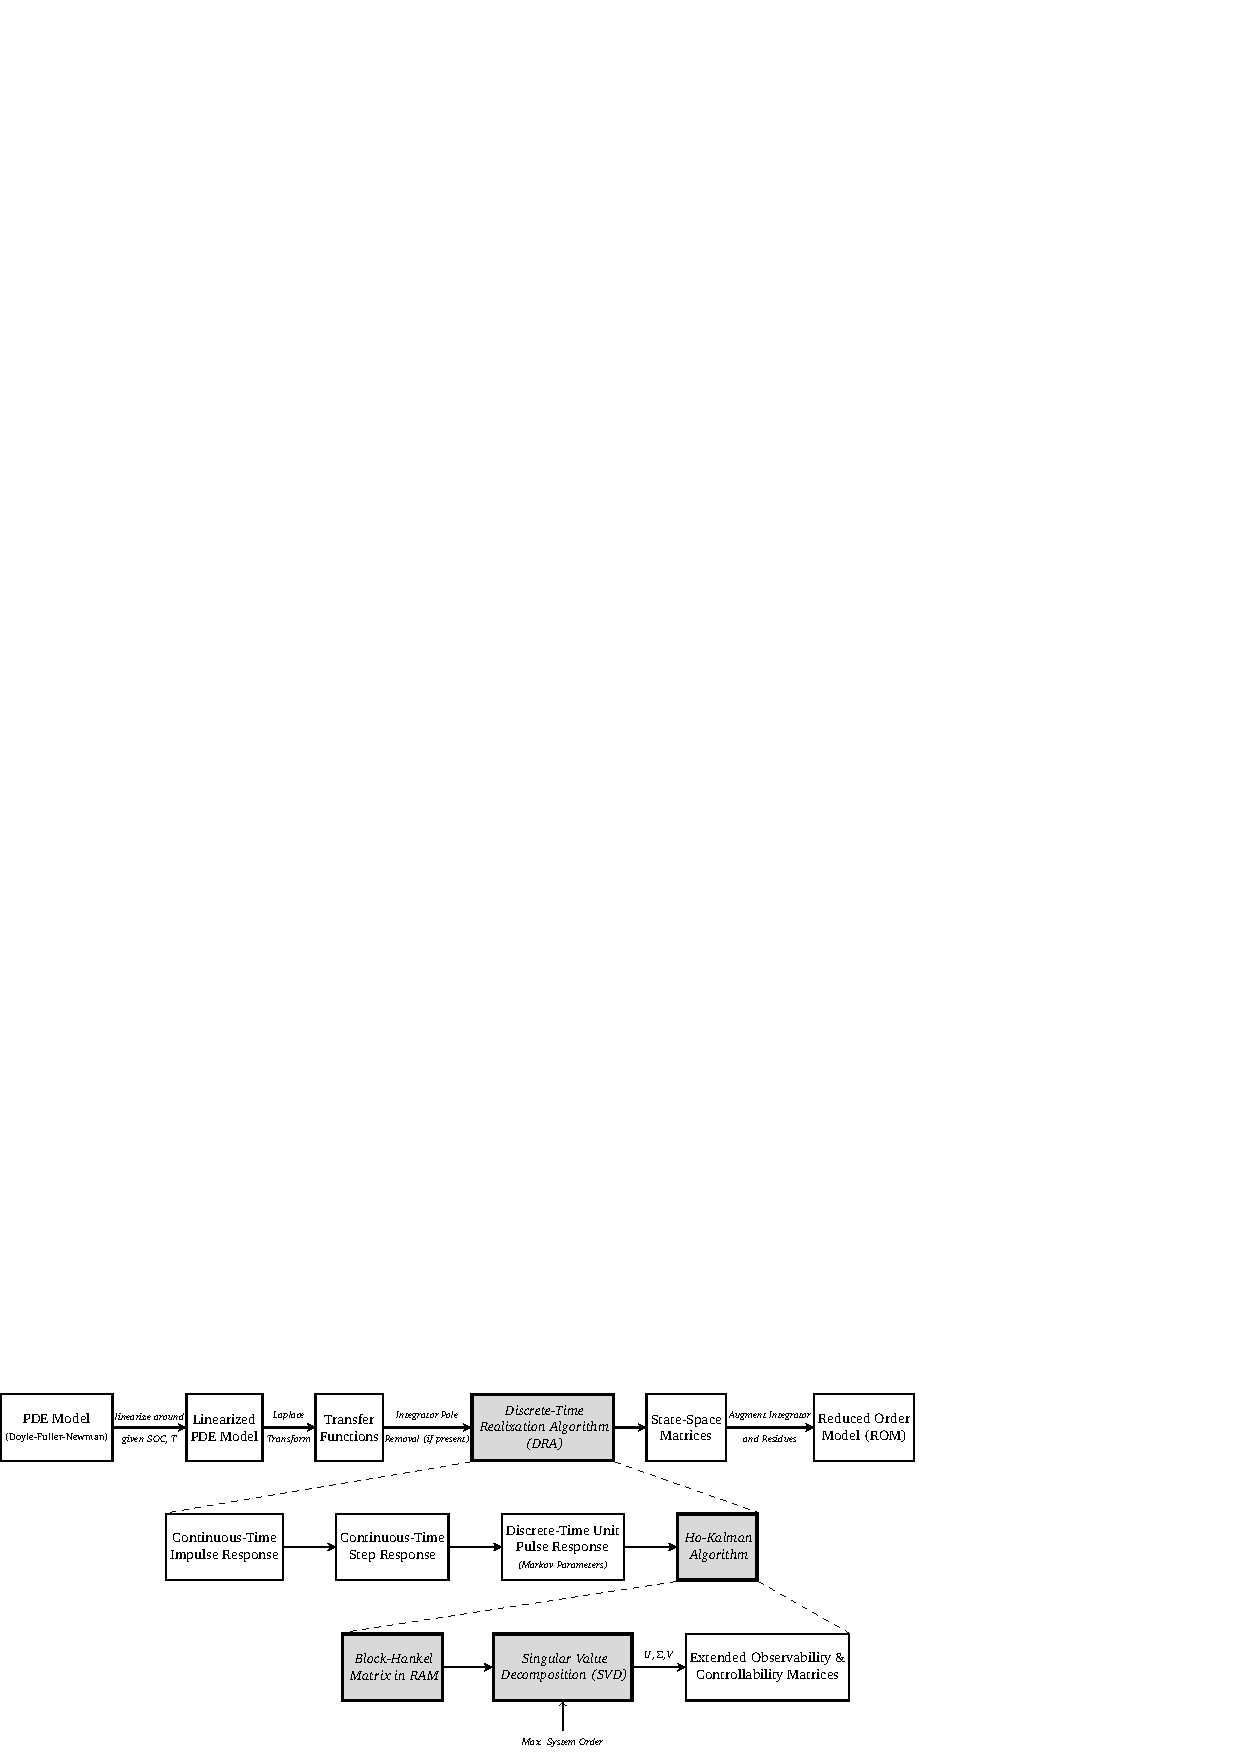
\includegraphics[width=\textwidth]{traditional_dra.pdf}
    \caption[%
    \glsfmtshort{rom} workflow using classical \glsfmtshort{dra}.
    ]%
    {%
        Reduced-order modelling (ROM) workflow using classical
        \glsfmtshort{dra}. The shaded blocks represent computational bottlenecks.
    }%
    \label{fig:traditional_ROM_Workflow}
\end{figure}

\subsection{Size of the Block-Hankel Matrix}\label{sec:size-of-the}

Large Block-Hankel matrices can occur in \gls{dra} computation due to the
following reasons.
\begin{enumerate}
    \item
        For  a  given   duration  of  Markov-parameter  recording,   if  a  high
        sample-rate   \gls{rom}  is   desired,   the   emulation  frequency   in
        the   \gls{dra}  scheme   has   to  be   proportionately  increased   to
        accurately  compute  the continuous-time  step  and  pulse responses  in
        \cref{fig:traditional_ROM_Workflow}. This implies  that the total number
        of time-samples~$N$  for each  Markov parameter will  have to  be scaled
        linearly to  capture the  desired duration  of the  unit-pulse response.
        However,  the size  of the  Block-Hankel matrix  has a  \emph{quadratic}
        dependence on the Markov parameter length.
    \item
        The  recorded sample  size~$N$ could  also  become large  if the  Markov
        parameters of just  one of the transfer functions decay  very slowly. In
        Li-ion batteries, diffusion  within the solid particle  is typically the
        slowest process.  For the cell  modelled in Lee~\etal{},  the unit-pulse
        response of surface concentration of Li adjacent to the positive current
        collector  requires approximately  16000~samples before  reducing to  an
        appreciably low value, as shown in~\cref{fig:markov_cse_pos}.
    \item
        For  a  battery  modelling   problem  consisting  of  multiple  transfer
        functions,  the  number  of  entries in  the  Block-Hankel  matrix  also
        scales linearly  with the  number of transfer  functions. Thus,  if more
        cell  variables (\eg{}  concentrations and  potentials at  other spatial
        locations  within the  cell) are  to be  studied, then  the size  of the
        transfer function vector  and that of the  Block-Hankel matrix increases
        correspondingly.
\end{enumerate}

\begin{figure}[!htbp]
    \centering
    \includegraphics{markov_decay.pdf}
    \caption[Markov parameters of solid surface concentration at positive
    current collector]{Time evolution of Markov parameters of pole-removed transfer
        function corresponding to surface concentration of Li in the solid particle
    adjacent to positive current collector.}
    \label{fig:markov_cse_pos}
\end{figure}

Considering the combined  influence of these effects, if  $x$ transfer functions
are to  be modelled  and $N$  time-samples of  each Markov  parameter are  to be
captured, the corresponding size of the Block-Hankel matrix~$H$ is
\begin{equation}
    \text{Size}(H)\sim \mathcal{O}(x N^2)\text{ {entries}}
\end{equation}

This    has    a    significant     computational    impact    as    shown    in
\cref{subsec:Traditional-DRA--Memory} and \cref{subsec:Traditional-DRA--CPU}.

\subsection{Classical \glsfmtshort{dra} --- Memory (\glsfmtshort{ram}) Requirements}\label{subsec:Traditional-DRA--Memory}

Lee~\etal~\cite{Lee2012a}  modelled 28~transfer  functions representing  various
electrochemical  variables at  the current  collector and  separator interfaces.
Each Markov  parameter is  a 28~element  column vector.  16000~time-samples were
obtained at  a sample-rate of  \SI{1}{\hertz}, allowing sufficient time  for the
Markov parameters of  the slowest dynamics \ie{} solid  surface concentration to
settle to an  acceptably low magnitude. The Block-Hankel matrix  thus formed has
8000~blocks,  each  block  consisting  of 28~elements  \ie{}  has  $8000  \times
28=224000$~rows  and 8000~columns.  Hence,  the overall  number  of elements  in
the  Block-Hankel  matrix is  $224000  \times  8000=1.79 \times  10^{9}$.  Using
double-precision  arithmetic, its  storage requirement  can be  estimated to  be
\approx \SI{27}{\giga\byte}.

Computing the \gls{svd} results in the formation of three more large matrices in
memory ---
\begin{enumerate*}[label=\roman*)]
    \item matrix   of   output  singular   vectors~$U$,
    \item matrix of  input  singular vectors~$V$, and
    \item the diagonal singular-value  matrix~$\Sigma$.
\end{enumerate*}
With  8000~Hankel-blocks,  approximately  \SI{81}{\giga\byte}  of  \gls{ram}  is
required for holding these three output  matrices generated by a full \gls{svd}.
However,  the  intermediate  operational   memory  usage  during  the  \gls{svd}
computation is often much higher than the  combined size of all the matrices. As
these large  matrices must  be repeatedly  handled for  each operating  point of
\gls{soc} and  temperature, the  high memory demand  of the  classical \gls{dra}
remains a persistent issue.

\subsection{Classical \glsfmtshort{dra} --- \glsfmtshort{cpu} Operation Count}\label{subsec:Traditional-DRA--CPU}

The most  widely used numerical  algorithm for  computing the full  \gls{svd} of
a  generic  dense  matrix $\mbox{\ensuremath{A\in\mathbb{R}^{m  \times  n},m\geq
n}}$  is  the  two-stage  Golub-Kahan-Reinsch  method~\cite{Golub2013}.  In  the
first  stage $A\in\mathbb{R}^{m  \times n}$  is reduced  to an  upper bidiagonal
form.  In  the  second  stage,   \gls{svd}  of  this  upper  bidiagonal  matrix,
$B\in\mathbb{R}^{m  \times n}$  is computed  using an  iterative procedure  such
as  the Demmel-Kahan  method~\cite{Golub2013}. If  stage~\romanletter{1} of  the
\gls{svd}  computation employs  $\mathbb{R}$-Bidiagonalization~\cite{Golub2013},
then the overall  process is referred to as $\mathbb{R}$-\gls{svd}.  This is the
fastest known  full \gls{svd}  computation method  that may  be applied  to this
battery modelling problem. The \textsc{dgesvd} algorithm, originally implemented
in  \textsc{LAPACK}~\cite{Anderson1999},  employs  this method.  This  has  been
ported to  many numerical computation  packages such  as MATLAB, GNU  Octave and
Scilab.  Several  numerical  libraries  such  as NAG  and  Intel  MKL  also  use
the  \textsc{dgesvd}  codes  due  to its  acclaimed  stability,  robustness  and
versatility.  The MATLAB  implementation `\texttt{\textbf{svd}}'  is also  based
upon \textsc{dgesvd} and  hence this can be considered as  the de-facto baseline
\gls{svd} code.

The    operation    count    for    computing   the    singular    values    and
vectors   of  a   generic   dense  matrix   $\mbox{\ensuremath{A\in\mathbb{R}^{m
\times   n},m\geq    n}}$   using    the   $\mathbb{R}$-\gls{svd}    method   is
$\mbox{\ensuremath{4m^{2}n+22n^{3}}}$~\cite{Golub2013}.  Markov   parameters  of
$x$~transfer functions  and $N$~time-samples  yields a Block-Hankel  matrix with
$m=x N$ rows and $n=N$ columns. Hence,
\begin{alignat}{2}
    \text{\glsfmtshort{cpu} Operation  Count} & = & \,4\left(xN\right){}^{2}N+22N^{3}\nonumber \\
                                              & = & \,2N^{3}\left(11+2x^{2}\right)\label{eq:cpu_op_count}
\end{alignat}
Thus  the \gls{cpu}  operation  count scales  as  $\mathcal{O}(N^{3})$ with  the
number of Markov time-samples~$N$ and as $\mathcal{O}(x^{2})$ with the number of
transfer  functions~$x$ being  modelled. The  \gls{rom} computed  in Lee~\etal{}
uses  28~transfer functions  wherein  the Markov  parameters  are collected  for
\SI{16000}{\second}  with  a sampling  interval  of  \SI{1}{\second}. Thus,  the
\gls{cpu}  operation  count for  performing  this  computation is  approximately
$\mathcal{O}(16000^{3})\approx 4 \times 10^{12}$ floating point operations.

\subsection{Summary Effect of Computational Bottlenecks}\label{subsec:Summary-Effect-of}

The computational bottleneck in a  classical \gls{dra} implementation arises due
to the  requirement of capturing a  large number of Markov  parameters, which in
turn leads  to growth in  Block-Hankel size. In  the case of  battery modelling,
this can arise in the following real-life scenarios:
\begin{enumerate}
	\item
        Electrochemical variables at additional locations of interest within the
        cell (\eg{}  middle of electrode or  separator domain) might need  to be
        modelled. This increases the number  of transfer functions and hence the
        number of Markov parameters.
	\item
        High frequency load  cycles necessitate higher sample-rates  to obtain a
        high fidelity  model. This leads  to a correspondingly higher  number of
        Markov parameters.
	\item
        In cells with  large particle sizes and small  diffusion coefficients, a
        large set  of Markov  parameters is  needed to  capture the  full system
        dynamics.
\end{enumerate}
Lack  of  specialized  computing infrastructure  necessitates  early  truncation
of  the  Markov parameters  in  the  \gls{rom}  workflow. The  resulting  errors
in  the singular  value  computation  lead to  significant  modelling errors  in
the  physical  variables of  the  cell.  Thus,  in practice,  the  computational
bottlenecks of classical \gls{dra} manifest as modelling errors when implemented
in  a  resource-constrained  computing environment.  Furthermore,  this  tedious
computation has to be repeated for multiple \glspl{soc} and temperatures.

The foregoing analysis  clearly demonstrates that the high  memory and \gls{cpu}
demands in  a classical \gls{dra}  implementation severely hamper the  scope and
applicability  of the  reduced order  modelling process.  This implies  that the
modelling  workflow is  not accessible  to research  groups without  specialized
computing infrastructure and its universal  appeal is rendered questionable. The
shaded  blocks in  \cref{fig:traditional_ROM_Workflow}  depict the  hierarchical
propagation of the classical \gls{dra}'s computational bottleneck throughout the
\gls{rom} workflow.

\section{Improved \glsfmtshort{dra} for Battery Modelling}\label{sec:Efficient-Computation-of}

Collecting a  large Markov parameter  set is  inevitable due to  the fundamental
physics of the cell  dynamics as established in \cref{subsec:Summary-Effect-of}.
Hence, in  order to circumvent the  high computational demands of  the classical
\gls{dra}, the second step in the process \ie{} forming the Block-Hankel matrix,
is critically examined with the following scientific rationale.

\begin{enumerate}
	\item
        The unit-pulse responses of most  battery transfer functions (other than
        those of rate-limiting  steps such as solid  diffusion) decay relatively
        quickly. Hence it is inefficient to  record the Markov parameters of the
        full  system for  the  entire  duration needed  to  capture the  slowest
        dynamics.
	\item
        The Block-Hankel  matrix is essentially redundant  information since its
        entries are simply the Markov parameters arranged in a repeating special
        structure. Thus,  it is wasteful to  construct this huge matrix.  If the
        \gls{svd} operation  can be  performed on a  virtual Hankel  matrix, the
        memory requirements can be drastically reduced.
	\item
        The matrix of singular values~$\Sigma$ is diagonal and hence, sparse. It
        is redundant to hold all the non-diagonal entries (zeros) in memory.
	\item
        It  is not  necessary to  perform a  \emph{full} \gls{svd}  operation in
        order  to  achieve order  reduction.  When  an  upper bound  on  desired
        system order  can be  decided a  priori, it is  sufficient to  compute a
        \emph{truncated} \gls{svd}  yielding the first few  dominant triplets of
        $U, \Sigma \text{ and } V$.
\end{enumerate}
Thus,  forming the  large Block-Hankel  matrix  and computing  its \gls{svd}  is
identified as an avoidable bottleneck in the classical \gls{dra}method. This can
be  tackled since  forming the  Block-Hankel matrix  is an  idiosyncrasy of  the
algorithm  used  and  does  not  arise from  any  fundamental  physical  limits.
Facilitated  by  an  efficient  \gls{svd}  implementation,  this  thesis  author
proposes  an improved  \gls{dra}that  serves  as a  drop-in  replacement in  the
\gls{rom} workflow.

\subsection{Candidate Schemes for Block-Hankel \glsfmtshort{svd}}

Generic  \gls{svd}  routines  such  as \textsc{dgesvd}  do  not  take  advantage
of  the  anti-diagonal  structural  symmetry  of  Block-Hankel  matrices.  Since
it  is sufficient  to  obtain  the first  few  leading  eigentriplets for  order
reduction,  iterative  algorithms  such  as   the  Jacobi  and  Lanczos  schemes
(see~\cite{Golub2013}  emerge  as  attractive  candidates  for  computing  these
dominant singular  values and vectors. In  order to ensure accessibility  to the
large community of  battery researchers and to encourage  widespread adoption of
the fast reduced order modelling framework, the author of this thesis considered
only freely available  open-source numerical libraries that exist  in the public
domain, especially  those with permissive  licensing terms. Otherwise  the gains
achieved by  an efficient  \gls{svd} computation  for implementing  \gls{dra} on
non-specialized  computing  hardware would  be  offset  by commercial  licensing
terms,  usage restrictions  and  monetary considerations  associated with  using
proprietary  codes. Among  these  open-source candidate  algorithms, the  Jacobi
scheme~\cite{Golub2013} is  available through the  xGESVD routine in  the LAPACK
suite~\cite{Anderson1999}. FORTRAN 77 codes for the implicitly restarted Arnoldi
and Lanczos schemes~(see~nu-TrLan~\cite{Yamazaki2008}) are  available as part of
the ARPACK~\cite{Lehoucq1998} library.

The practical drawback  of most \gls{svd} implementations,  both open-source and
proprietary, is  that they require  the entire  matrix as input  argument. Since
operating upon  the Block-Hankel  matrix requires constructing  it in  the first
place, the memory bottlenecks discussed in \cref{subsec:Traditional-DRA--Memory}
are  not  ameliorated. An  example  is  the  \texttt{svds} routine,  an  economy
size  \gls{svd}   implementation  in  MATLAB.   Albeit  this  is   a  commercial
implementation  of  the  Arnoldi  codes,  any potential  benefits  of  using  an
iterative scheme is nullified by the memory penalty. Owing to reasons enumerated
in \cref{sec:Efficient-Computation-of}, the chosen  \gls{svd} algorithm needs to
be able to handle the computation without actually forming the huge block-Hankel
matrix in memory.

% \subsection{\gls{svd} Operation on a Virtual Block-Hankel Matrix}

% R.M. Larsen's pioneering work PROPACK~\cite{Larsen2014} implements
% a numerically stable Lanczos \gls{svd} computation designed specifically
% for large and sparse matrices. In addition to the ability to operate
% on the matrix as a whole, the PROPACK codes possess a unique flexibility
% of accepting input arguments in functional form. A key highlight of
% the Lanczos \gls{svd} scheme is that it does not strictly require the matrix
% itself, but only the product of the matrix and its transpose with
% an arbitrary vector. This feature has been effectively exploited in
% the PROPACK suite. Therefore, these multiplication routines can be
% supplied as input arguments instead of forming the large Block-Hankel
% matrices in memory. Furthermore, this package includes sophisticated
% schemes such as Gram-Schmidt partial re-orthogonalization~\cite{Bjoerck1994}
% to compensate for numerical round-off errors in the basic Lanczos
% bidiagonalization and ensures orthogonality of the input and output
% singular vectors. The PROPACK suite is available as both Fortran 77
% and MATLAB codes distributed under a permissive BSD license~\cite{Rosen2005}.

% For the \gls{rom} workflow, in order to use PROPACK's unique feature, i.e.
% its flexibility to accept functional form inputs, the key is to use
% an algorithm that effectively exploits the affine structure of the
% Block-Hankel matrix without actually forming it in memory. Recent
% research in a specialized time-series technique known as Singular
% Spectrum Analysis (SSA)~\cite{ElsnerTsonis2013} has yielded efficient
% methods for achieving this goal. Korobeynikov~\cite{Korobeynikov2009}
% proposed an algorithm that employs the Fast Fourier Transform (FFT)
% for implementing this matrix-vector product by embedding the Markov
% parameters into the column vectors of a circulant matrix. This is
% suitable for applications wherein the Hankel matrix is composed of
% scalar entries such as that formed by the Markov parameters of a single
% input single output (SISO) transfer function. Golyandina and Usevich~\cite{GolyandinaKorobeynikovShlemovEtAl2015,GolyandinaUsevich2004}
% extended this approach to a generic 2D-case for performing Singular
% Spectrum Analysis (SSA) on images. With this modification, this algorithm
% is rendered capable of handling the structure of Multi-level Block-Hankel
% matrices formed from the Markov parameters of a generic Multi-Input-Multi-Output
% (MIMO) system. While the modified scheme does not construct the Block-Hankel
% matrix in memory, the operational rubrics of the Golyandina-Usevich
% algorithm in conjunction with PROPACK is such that they iteratively
% operate on a virtual Hankel matrix of equivalent size. The Golyandina-Usevich
% algorithm is briefly summarized in Appendix \ref{sec:Golyandina-Usevich-Algorithm}.



% -*- root: ../main.tex -*-
%!TEX root = ../main.tex
% this file is called up by main.tex
% content in this file will be fed into the main document
% vim:textwidth=80 fo=cqt

In this  section, the  quadratic approximation  of ionic  spatial concentration,
that underpins the electrolyte model  in many improved \gls{spm} formulations is
presented. An analysis of  the weakness of this model is  performed based on the
results  from applying  this model.  Mitigation of  this critical  drawback lead
to  this  author's  decoupled spatio-temporal  electrolyte  concentration  model
structure which is presented next in~\cref{sec:newelectrolytemodel}.

\begin{figure}[!htb]
    \captionsetup{singlelinecheck=off}
    \centering
    \includegraphics{placeholder_images/example-image-golden.pdf}
    \caption[Co-ordinate systems for quadratic approximation of
    electrolyte concentration]{Schematic diagram of the electrochemical sandwich
        consisting of
        \begin{enumerate*}[label=\itshape\alph*\upshape)]
            \item negative electrode,
            \item separator, and
            \item positive electrode
        \end{enumerate*} depicting the co-ordinate system used in deriving the
        quadratic approximation profile. The global spatial co-ordinate is $x
        \in \{0,l_\text{tot}\}$, where $l_\text{tot} = l_\text{neg} +
        l_\text{sep} + l_\text{pos}$. Local co-ordinate systems specific to each
        region are also defined. It should be noted that the positive
        electrode's local co-ordinate axis direction is reversed.}
    \label{fig:coordsquadapprox}
\end{figure}

The  schematic  in~\cref{fig:coordsquadapprox}  shows   the  definition  of  the
co-ordinate  systems  used  in  deriving the  polynomial  approximation  of  the
electrolyte concentration  profile. The globally defined  $x$ co-ordinate starts
at  the negative  current  collector  interface ($x=0$)  and  terminates at  the
positive  current  collector  interface  ($x =  l_\text{tot},\,  l_\text{tot}  =
l_\text{neg} +  l_\text{sep} +  l_\text{pos}$). Three local  co-ordinate systems
$z_\mu$  valid  only  within  their  respective regions  are  also  defined.  In
particular, it  must be  noted that  the direction  of the  local $z_\text{pos}$
co-ordinate axis is opposite to that of  the other two local co-ordinate axes as
well as the global co-ordinate axis. In subsequent usages, the suffix in $z_\mu$
is dropped and  the reader is advised  to infer the region of  validity from the
usage  context  which are  unambiguous  as  they  occur in  separate  equations.
Furthermore, the  notation of  the three regions  $\{\text{neg, sep,  pos}\}$ is
abbreviated  to $\{n,s,p\}$  respectively in  all mathematical  expressions. The
author  is convinced  that this  notation does  not detract  from following  the
derivations, but rather aids it by keeping the notations compact.

A  standard  quadratic expression  is  chosen  a  priori for  approximating  the
electrolyte concentration profile within each region.
\begin{alignat}{2}
    c_\ensub &= a_2(t) z^2 + a_1(t) z + a_0(t),\quad &&0 \le z \le l_\text{n}\label{eq:cenquadstart} \\
    c_\essub &= a_5(t) z^2 + a_4(t) z + a_3(t),\quad &&0 \le z \le l_\text{s}\label{eq:cesquadstart} \\
    c_\epsub &= a_8(t) z^2 + a_7(t) z + a_6(t),\quad &&0 \le z \le l_\text{p}\label{eq:cepquadstart}
\end{alignat}
where  the  coefficient  vector  $\vect{a_0(t),a_1(t),  \dots  ,a_8(t)}$  is  to
be   determined   at   each   time-step\footnote{For   brevity,   in   rest   of
the   equations,   the   time-dependence   is   dropped   from   the   notation.
However,  it   must  be   implicitly  understood   that  all   coefficients  are
indeed  time-varying.}.   Applying  boundary   conditions  of   the  electrolyte
diffusion  equation  of   the  \gls{dfn}  model~(refer  \cref{eq:dfnliquiddiff})
to~\crefrange{eq:cenquadstart}{eq:cepquadstart}, it is clear  that $a_1 = 0$ and
$a_7 = 0$. Thus, ~\crefrange{eq:cenquadstart}{eq:cepquadstart} become
\begin{alignat}{2}
    c_\ensub &= a_2(t) z^2 + a_0(t),\quad &&0 \le z \le l_\text{n}\label{eq:cenquadreduced} \\
    c_\essub &= a_5(t) z^2 + a_4(t) z + a_3(t),\quad &&0 \le z \le l_\text{s}\label{eq:cesquadreduced} \\
    c_\epsub &= a_8(t) z^2 + a_6(t),\quad &&0 \le z \le l_\text{p}\label{eq:cepquadreduced}
\end{alignat}

% -*- root: ../../main.tex -*-
%!TEX root = ../../main.tex
% this file is called up by main.tex
% content in this file will be fed into the main document
% vim:nospell textwidth=180 foldlevelstart=3 foldlevel=3 conceallevel=0

\begin{table}[!htbp]
    \centering
    \caption[Electrolyte equations \& boundary conditions of \glsfmtshort{dfn} model in separator]{Electrolyte-specific governing equations and boundary conditions of the \glsfmtlong{dfn}~(\glsfmtshort{dfn}) model within the separator domain.}
    \label{tbl:dfnelectrolyteeqnsinsep}
    \begingroup
    \makeatletter\def\f@size{9.25}\check@mathfonts
    \addtolength{\jot}{0.875em}
    \begin{tabular*}{\textwidth}{@{} l c r l r @{}}
        \toprule
        \multicolumn{1}{c}{\small Region} & \small Governing equations & \multicolumn{2}{c}{\small Boundary conditions } & {} \\
        {} & {} & \multicolumn{2}{c}{\scriptsize $(l_\text{neg} \coloneqq l_\text{n},\, l_\text{sep} \coloneqq l_\text{s},\, l_\text{pos} \coloneq l_\text{p})$} \\
        \midrule
        \multicolumn{1}{l |}{{\rotatebox[origin=c]{90}{\makecell{\footnotesize Separator\\ \scriptsize $\delta \in \{\text{sep}\}$}}}} &
        $\begin{aligned}
            \vphantom{D_{\text{\tiny eff}_\text{n}}\!\! \! \!\, \diffp{c_\text{e}}{x}{\mathrlap{x = l^{-}_\text{n}}}} \varepsilon_\delta \diffp{c_\text{e}}{t} &=D_\effdelta  \diffp[2]{c_\text{e}}{x} \\[-0.75em]
            \vphantom{D_{\text{\tiny eff}_\text{s}}\!\! \! \!\, \diffp{c_\text{e}}{x}{\mathrlap{x=(l_{\text{n}} + l_\text{s})^{-}}}}\\[1.25em]
            \vphantom{\kappa_{\text{\tiny eff}_\text{n}}\!\! \! \!\, \diffp{c_\text{e}}{x}{\mathrlap{x = l^{-}_\text{n}}}\hspace{5mm} =\kappa_{\text{\tiny eff}_\text{s}}\!\!\!\!\,\diffp{c_\text{e}}{x}{\mathrlap{x = l^{+}_\text{n}}}} \frac{I}{A} &= \overline{\kappa}_\effdelta \left( \diffp[2]{\phi_\text{e}}{x} + \frac{2 R T}{F} (t^0_{+}-1)\diffp[2]{ \ln c_\text{e}}{x}\right) \\[-0.75em]
            \vphantom{\kappa_{\text{\tiny eff}_\text{s}}\!\! \! \!\, \diffp{c_\text{e}}{x}{\mathrlap{x=(l_{\text{n}} + l_\text{s})^{-}}}} \\
        \end{aligned}$ &
        $\begin{aligned}
    \vphantom{D_{\text{\tiny eff}_\text{n}}\!\! \! \!\, \diffp{c_\text{e}}{x}{\mathrlap{x = l^{-}_\text{n}}}} \qquad c_\text{e}\Bigr\rvert_{\mathrlap{x=l^{-}_\text{n}}}\hspace{5mm} &= c_\text{e}\Bigr\rvert_{\mathrlap{x=l^{+}_\text{n}}},\\[-0.75em]
     \vphantom{\kappa_{\text{\tiny eff}_\text{n}}\!\! \! \!\, \diffp{c_\text{e}}{x}{\mathrlap{x = l^{-}_\text{n}}}\hspace{5mm} =\kappa_{\text{\tiny eff}_\text{s}}\!\!\!\!\,\diffp{c_\text{e}}{x}{\mathrlap{x = l^{+}_\text{n}}}} c_\text{e}\Bigr\rvert_{\mathrlap{x=(l_{\text{n}} + l_\text{s})^{-}}}\hspace{5mm} &= c_\text{e}\Bigr\rvert_{\mathrlap{x=(l_{\text{n}} + l_\text{s})^{+}}},\\[1.25em]
 \vphantom{\kappa_{\text{\tiny eff}_\text{n}}\!\! \! \!\, \diffp{c_\text{e}}{x}{\mathrlap{x = l^{-}_\text{n}}}} \vphantom{\left( \diffp[2]{\phi_\text{e}}{x} + \frac{2 R T}{F} (t^0_{+}-1)\diffp[2]{ \ln c_\text{e}}{x}\right)} \phi_\text{e}\Bigr\rvert_{\mathrlap{x=l^{-}_\text{n}}}\hspace{5mm} &= \phi_\text{e}\Bigr\rvert_{\mathrlap{x=l^{+}_\text{n}}},\\[-0.75em]
 \vphantom{\kappa_{\text{\tiny eff}_\text{s}}\!\! \! \!\, \diffp{c_\text{e}}{x}{\mathrlap{x=(l_{\text{n}} + l_\text{s})^{-}}}} \phi_\text{e}\Bigr\rvert_{\mathrlap{x=(l_{\text{n}} + l_\text{s})^{-}}}\hspace{5mm} &= \phi_\text{e}\Bigr\rvert_{\mathrlap{x=(l_{\text{n}} + l_\text{s})^{-}}},\\
    \end{aligned}$ &
    $\begin{aligned}
        \quad D_{\text{\tiny eff}_\text{n}}\!\! \! \!\, \diffp{c_\text{e}}{x}{\mathrlap{x = l^{-}_\text{n}}}\hspace{5mm} &=D_{\text{\tiny eff}_\text{s}}\!\!\!\!\,\diffp{c_\text{e}}{x}{\mathrlap{x = l^{+}_\text{n}}}\\[-0.75em]
        D_{\text{\tiny eff}_\text{s}}\!\! \! \!\, \diffp{c_\text{e}}{x}{\mathrlap{x=(l_{\text{n}} + l_\text{s})^{-}}}\hspace{5mm} &=D_{\text{\tiny eff}_\text{p}}\!\!\!\!\,\diffp{c_\text{e}}{x}{\mathrlap{x=(l_{\text{n}} + l_\text{s})^{+}}}\\[1.25em]
        \vphantom{\left( \diffp[2]{\phi_\text{e}}{x} + \frac{2 R T}{F} (t^0_{+}-1)\diffp[2]{ \ln c_\text{e}}{x}\right)} \kappa_{\text{\tiny eff}_\text{n}}\!\! \! \!\, \diffp{c_\text{e}}{x}{\mathrlap{x = l^{-}_\text{n}}}\hspace{5mm} &=\kappa_{\text{\tiny eff}_\text{s}}\!\!\!\!\,\diffp{c_\text{e}}{x}{\mathrlap{x = l^{+}_\text{n}}}\\[-0.75em]
        \kappa_{\text{\tiny eff}_\text{s}}\!\! \! \!\, \diffp{c_\text{e}}{x}{\mathrlap{x=(l_{\text{n}} + l_\text{s})^{-}}}\hspace{5mm} &=\kappa_{\text{\tiny eff}_\text{p}}\!\!\!\!\,\diffp{c_\text{e}}{x}{\mathrlap{x=(l_{\text{n}} + l_\text{s})^{+}}}\\
    \end{aligned}$ &
    $\begin{aligned}
        \vphantom{D_{\text{\tiny eff}_\text{n}}\!\! \! \!\, \diffp{c_\text{e}}{x}{\mathrlap{x = l^{-}_\text{n}}}} \quad \refstepcounter{equation}(\theequation)\label{eq:liquiddiffnsep} \\[-0.75em]
        \vphantom{D_{\text{\tiny eff}_\text{s}}\!\! \! \!\, \diffp{c_\text{e}}{x}{\mathrlap{x=(l_{\text{n}} + l_\text{s})^{-}}}}\\[1.25em]
        \vphantom{\kappa_{\text{\tiny eff}_\text{n}}\!\! \! \!\, \diffp{c_\text{e}}{x}{\mathrlap{x = l^{-}_\text{n}}}} \vphantom{\left( \diffp[2]{\phi_\text{e}}{x} + \frac{2 R T}{F} (t^0_{+}-1)\diffp[2]{ \ln c_\text{e}}{x}\right)} \refstepcounter{equation}(\theequation) \label{eq:liquidpotentialsep}\\[-0.75em]
        \vphantom{\kappa_{\text{\tiny eff}_\text{s}}\!\! \! \!\, \diffp{c_\text{e}}{x}{\mathrlap{x=(l_{\text{n}} + l_\text{s})^{-}}}}
    \end{aligned}$
    \\
    \bottomrule
\end{tabular*}
\endgroup
\end{table}



\Cref{tbl:dfnelectrolyteeqnsinsep}    lists   the    equations   and    boundary
conditions   for  phenomena   describing   electrolyte   diffusion  and   charge
balance  within  the   separator  domain.  Essentially,~\cref{eq:liquiddiffnsep}
and~\cref{eq:liquidpotentialsep}  are  obtained  by applying  the  corresponding
electrolyte  equations  of  the \gls{dfn}  model  (see  ~\cref{eq:dfnliquiddiff}
and~\cref{eq:dfnliquidpotential}) respectively to the separator region.


\cleardoublepage

\begin{appendices} % Using appendices environment for more functionality
    \crefalias{chapter}{appchap}
    % -*- root: ../main.tex -*-
%!TEX root = ../main.tex
% ******************************* Thesis Appendix A ****************************
\chapter{Appendix A }

\end{appendices}

\backmatter

\begin{footnotesize} % tiny(5) < scriptsize(7) < footnotesize(8) < small (9)
    \renewcommand{\bibname}{References} % changes the header; default: Bibliography
    % add bib to toc
    \cleardoublepage
    \phantomsection
    \addcontentsline{toc}{chapter}{\bibname}
    \printbibliography
\end{footnotesize}
\batchmode
\end{document}
